%============================================================================
% tento soubor pouzijte jako zaklad
% (c) 2008 Michal Bidlo
% E-mail: bidlom AT fit vutbr cz
%============================================================================
% kodovaní: utf-8 (zmena prikazem iconv, recode nebo cstocs)
%----------------------------------------------------------------------------
% zpracování: make, make pdf, make desky, make clean
% připomínky posílejte na e-mail: bidlom AT fit.vutbr.cz
% vim: set syntax=tex encoding=latin2:
%============================================================================
\documentclass[english]{fitthesis} % odevzdani do wisu - odkazy, na ktere se da klikat
%\documentclass[print, english]{fitthesis} % pro tisk - na odkazy se neda klikat


% zde zvolime kodovani, ve kterem je napsan text prace
% "latin2" pro iso8859-2 nebo "cp1250" pro windows-1250, "utf8" pro "utf-8"
%\usepackage{ucs}
\usepackage[T1,IL2]{fontenc}
\usepackage[utf8]{inputenc}
\usepackage{url}
\DeclareUrlCommand\url{\def\UrlLeft{<}\def\UrlRight{>} \urlstyle{tt}}

% doplnujici prikazy
% ----------------------------------------------

% todo oznacuje cast, ktere je se musi dodelat
\newcommand{\todo}[1][something needs to be done in here\ldots]{\textcolor{red}{TODO: #1}}

% phony se da vzuzit pro poznamky - sazi se sede
\newcommand{\phony}[1]{\textcolor{gray}{#1}}

% blind je zobrazi X odstavcu tupeho textu - vhodne pro simulovani delky jednotlivych casti
\usepackage{blindtext}
\newcommand{\blind}[1]{\textcolor{gray}{\Blindtext[#1]}}

\newcommand{\insertImg}[4][1.0]{
\begin{figure}[ht]
	\centering
	\includegraphics[width=#1\linewidth]{fig/#2}
	\caption{#3}
	\label{#4}
\end{figure}
}

\usepackage{float}
\newcommand{\insertImgHere}[4][1.0]{
\begin{figure}[H]
	\centering
	\includegraphics[width=#1\linewidth]{fig/#2}
	\caption{#3}
	\label{#4}
\end{figure}
}

\newcommand{\todoImg}[1][0.5]{\insertImg[#1]{placeholder.pdf}{\todo[Replace with real image\ldots]}{todo}}


% Pouzita literatura
% ----------------------------------------------
\ifczech
  \usepackage[backend=biber, style=czechiso]{biblatex}
\else 
  \usepackage[backend=biber, style=trad-plain]{biblatex}
  %\usepackage[backend=biber, style=trad-alpha]{biblatex}
\fi


\addbibresource{literatura.bib}
\addbibresource{rfc.bib}

%zde muzeme vlozit vlastni balicky
%%%%%%%%%%%%%%%%%%%%%%%%%%%%%%%%%%%%%%%%%%%%%%%%%%%%%%%%%%%%%%%%%%%%%
% put \usepackage inside
%%%%%%%%%%%%%%%%%%%%%%%%%%%%%%%%%%%%%%%%%%%%%%%%%%%%%%%%%%%%%%%%%%%%%
\usepackage{tikz}

\usepackage{perpage} % the perpage package
\MakePerPage{footnote} % the perpage package command

\usepackage{wrapfig} % wrapping of figures

\usepackage{etoolbox} % tools for commands changing
\patchcmd{\listoffigures}{\chapter*}{\chapter}{}{} % use \chapter instead of \chapter* for list of figures

\usepackage{color} % color macros
\definecolor{pblue}{rgb}{0.13,0.13,1}
\definecolor{pgreen}{rgb}{0,0.5,0}
\definecolor{pred}{rgb}{0.9,0,0}
\definecolor{pgrey}{rgb}{0.46,0.45,0.48}

\usepackage{csquotes} % advanced capabilities for inline and block quotes
\usepackage{graphicx} % including graphics
\usepackage{pdfpages} % simply including pdf files
\usepackage[bottom]{footmisc} % aligning footnotes to bottom
\usepackage{listings} % listings for CODE writing

\usepackage{cleveref} % clever referencing

% setting of Java language for listing environment
\lstset{language=Java,
  showspaces=false,
  showtabs=false,
  breaklines=true,
  showstringspaces=false,
  breakatwhitespace=true,
  commentstyle=\color{pgreen},
  keywordstyle=\color{pblue},
  stringstyle=\color{pred},
  basicstyle=\ttfamily,
  moredelim=[il][\textcolor{pgrey}]{$$},
  moredelim=[is][\textcolor{pgrey}]{\%\%}{\%\%}
} % viz. packages.tex

% =======================================================================
% balíček "hyperref" vytváří klikací odkazy v pdf, pokud tedy použijeme pdflatex
% problém je, že balíček hyperref musí být uveden jako poslední, takže nemůže
% být v šabloně
\ifWis
\ifx\pdfoutput\undefined % nejedeme pod pdflatexem
\else

  \usepackage{color}
  \usepackage[unicode,colorlinks,hyperindex,plainpages=false,pdftex]{hyperref}
  \definecolor{links}{rgb}{0.25,0.32,0.71}
  \definecolor{anchors}{rgb}{1,0,0}
  \def\AnchorColor{anchors}
  \def\LinkColor{links}
  \def\pdfBorderAttrs{/Border [0 0 0] }  % bez okrajů kolem odkazů
  \pdfcompresslevel=9
  
  \definecolor{mdindigo}{HTML}{3F51B5}
  \definecolor{mdred}{HTML}{F44336}
  \definecolor{mdgreen}{HTML}{4CAF50}
  \hypersetup{
	urlcolor=mdindigo,
	linkcolor=mdred,
	citecolor=mdgreen
  }
\fi
\fi



%Informace o praci/projektu
%---------------------------------------------------------------------------
\projectinfo{
  %Prace
  project=DP,            %typ prace BP/SP/DP/DR
  year=2015,             %rok
  date=\today,           %datum odevzdani
  %Nazev prace
  title.cs={Android IP kamera},  %nazev prace v cestine
  title.en={Android IP camera}, %nazev prace v anglictine
  %Autor
  author={Jan Chvála},   %jmeno prijmeni autora
  author.title.p=Bc., %titul pred jmenem (nepovinne)
  %author.title.a=PhD, %titul za jmenem (nepovinne)
  %Ustav
  department=UPGM, % doplnte prislusnou zkratku: UPSY/UIFS/UITS/UPGM
  %Skolitel
  supervisor={Adam Herout}, %jmeno prijmeni skolitele
  supervisor.title.p={doc. Ing.},   %titul pred jmenem (nepovinne)
  supervisor.title.a={Ph.D.},    %titul za jmenem (nepovinne)
  %Klicova slova, abstrakty, prohlaseni a podekovani je mozne definovat 
  %bud pomoci nasledujicich parametru nebo pomoci vyhrazenych maker (viz dale)
  %===========================================================================
  %Klicova slova
  keywords.cs={Real Time Communications, WebRTC, Android, Google Cloud Messaging, IP kamera}, %klicova slova v ceskem jazyce
  keywords.en={Real Time Communications, WebRTC, Android, Google Cloud Messaging, IP camera}, %klicova slova v anglickem jazyce
  %Abstract
  abstract.cs={
Cílem této práce je navrhnout systém, který by umožnil odesílání dat z videokamery mobilního zařízení a jejich zobrazení v reálném čase prostřednictvím webového prohlížeče. Součástí práce je popis použitých technologií a také popis cílové implementační platformy Android.
K řešení získání a přenosu multimediálních dat byla využita technologie Web Real Time Communications (WebRTC), která je nativně podporovaná novými prohlížeči a komponentou WebView (Android verze 5.0 a výše). Zasílání push notifikací ze strany serveru na mobilní zařízení pro spuštění streamu je řešeno pomocí Google Cloud Messaging technologie.
Výsledný systém umožňuje uživateli pomocí webového prohlížeče spustit aplikaci na mobilním telefonu a tím zahájit přenos multimediálních dat. Ten je možné parametrizovat a zabezpečit pomocí hesla.
Přínosem práce je seznámení s technologií WebRTC a demonstrace jejího snadného využití implementací IP kamery na platformě Android.
}, % abstrakt v ceskem jazyce
  abstract.en={
The goal of this thesis is to design a system which would allow video data streaming from a mobile device and real time playback using a standard web browser. The technological background and the implementation platform are both part of this thesis.
Web Real Time Communications (WebRTC) technology was used for acquiring multimedia data on mobile device. This technology is natively supported in the latest major web browsers and in WebView component (Android version 5.0 and above). Sending push notifications from a server to a mobile device to start the streaming is done with Google Cloud Messaging technology.
The resultant system allows a user to start the application on mobile device with easy web browser access. This starts the multimedia stream from device, which can be parametrized and secured by password.
The benefit of this thesis is the overview of WebRTC technology and its demonstration. The IP camera implementation shows how easy it is to use the WebRTC in real applications.
}, % abstrakt v anglickem jazyce
  %Prohlaseni
  declaration={Prohlašuji, že jsem tuto diplomovou práci vypracoval samostatně pod vedením pana doc.~Ing. Adama Herouta~Ph.D. a že jsem uvedl všechny literární prameny, ze kterých jsem čerpal.},
  %Podekovani (nepovinne)
  acknowledgment={Tímto bych rád poděkoval mému vedoucímu diplomové práce panu doc.~Ing. Adamu Heroutovi,~Ph.D., za pomoc při výběru a formování tématu, odborné konzultace a potřebnou motivaci.} % nepovinne
}

\begin{document}
  % Vysazeni titulnich stran
  % ----------------------------------------------
  \maketitle
  % Obsah
  % ----------------------------------------------
  \setcounter{tocdepth}{1}
  \tableofcontents
  
  % Seznam obrazku a tabulek (pokud prace obsahuje velke mnozstvi obrazku, tak se to hodi)
  %\listoffigures
  %\listoftables 

  % Text prace
  % ----------------------------------------------
  %=========================================================================
% This cahpter should introduce main goals of the thesis itself brief 
% description of the topic and the structure of the thesis.
\chapter{Introduction}
\label{chap:chapter1}
Last twenty years of technological innovation and development has brought us Internet Protocol (IP) cameras which are part of our everyday life. As a result of hardware cheapening the application of IP cameras is not restricted only for the enterprise usage but small companies, shops and even houses are protected with them more and more often. Anyone can buy expensive IP cameras or cheaper variations but there is no easy--to--use solution if you just want to test an IP camera without spending any money.

Software is also evolving very fast. The Web Real Time Communications (WebRTC) technology is being developed in recent years. The first technology of its kind for enabling peer--to--peer connection between two endpoints in the internet. It is still not yet completely standardized in the time of writing this thesis. But together with technological draft the reference implementation is developed as open--source project and major web browsers like Chrome, Firefox or Opera claim to support WebRTC or at least the main parts of it.

Mobile devices have the hardware necessities to be used as temporary IP cameras. The wireless connectivity is present and integrated cameras have sufficient resolution even for low cost devices. WebView (Android's native component with web browser engine) supports WebRTC technology for Android version 5.0 and above which makes it the right candidate for the mobile part of the resultant system.

This thesis will focus on exploration of this new technology for creating simple system for video streaming from Android device. The application will allow user to start the stream remotely by using Google Cloud Messaging (GCM) and view the stream on a web page. 

The beginning of the thesis (chapter \ref{chap:chapter2}) focuses on WebRTC which is the main implementation pillar for the resultant system. Then the Android Operating System and its relevant parts are described in chapter \ref{chap:chapter3}.
Chapter \ref{chap:chapter4} covers information about GCM technology used for sending messages from server to mobile application client.
Design of the resultant system and its implementation are described in chapter \ref{chap:chapter5}. Testing and measurements are in chapter \ref{chap:chapter6}.
The very last chapter \ref{chap:chapter7} summarize the results of this master thesis.

  %=========================================================================
% 
\chapter{Web Real Time Communications}
\label{chap:chapter2}
This chapter focuses on the Web Real Time Communications (WebRTC) technology which is the main pillar of the resultant system. WebRTC is a group of open standards which are being developed by World Wide Web Consorcium (W3C) and Internet Engineering Task Force (IETF). W3C is concentrating on JavaScript Application Programming Interface (API) which serves as a bridge between web application and Real Time Communications (RTC) function (see \ref{sec:rtc-function}). IETF is developing protocols used by RTC functions to communicate with each other. All the specifications are still actively developed in the time of writing this thesis but pre--standard implementation is already available as open--source project under the WebRTC name.

This technology allows to acquire local media data stream through simple API, connect to another endpoint in the internet and stream the multimedia data to it.

Knowledge base for most of the information is called "The WebRTC book" in it's third edition \cite{TheWebRTCBook}.




\section{Components}
The WebRTC technology is composed of a couple of components. This thesis focuses on web applications which are the main category where this technology should be used. Figure \ref{fig:figWebRTCArchitecture} shows how the WebRTC is placed in the web browser and WebRTC architecture itself. The important parts are Web API, which is the one we use in applications, RTC function, which handles peer--to--peer connection, and media engines for capturing user media.

\insertImg[0.79]{WebRTC-architecture.pdf}{WebRTC architecture and it's components.}{fig:figWebRTCArchitecture}



\subsection{Real Time Communications function}
\label{sec:rtc-function}
The most important part of WebRTC is RTC function module. This module is responsible for communication between other RTC functions using on--the--wire protocols\footnote{Such as Transmission Control Protocol (TCP) or User Datagram Protocol (UDP).} and for communication with operating system. Each RTC function is considered to be an endpoint in the World Wide Web (WWW) and in this thesis it will be also referred to as peer.


\subsubsection{Topologies}
%\subsection{Topologies}
The connection between peers can be established basically as two different topologies Triangle and Trapezoid. Triangle means that two peers are using the same web application on the same server\footnote{Triangle topology is what we will use in the resultant system.} while Trapezoid on the other hand is when each peer is using different web application (Figure~\ref{fig:figWebRTCTopology}) on a different server.

\insertImg[0.9]{WebRTC-topology.pdf}{WebRTC peer connection topology topology.}{fig:figWebRTCTopology}


\subsection{Signalling servers}
Signalling is not a part of WebRTC effort for standardization but it is intensively used for establishing peer--to--peer connection between two peers. It is described in section \ref{sec:webrtc-signalling}.

WebRTC uses technology to overcome common problems when communicating in WWW on top of signalling process. Usually most of the peers are hidden behind Network Address Translators (NAT)\footnote{Networking devices for translating local IP addresses to the one used as an endpoint to another network. For more information see \cite{rfc3022}}. In this case direct communication between peers behind different NATs is not possible.

\insertImg[1.0]{WebRTC-ice-real-world.pdf}{Direct peer--to--peer communication is not possible in real world.}{fig:iceRealWorld}

Interactive Connectivity Establishment (ICE) helps to deal with NATs and WebRTC and provides the ability to set up signalling so it can use ICE for NAT traversal. ICE uses Session Traversal Utilities for NAT (STUN) to gather all candidate addresses from both peers and systematically tries all possible pairs \cite{rfc5245} to establish peer--to--peer connection. Traversal Using Relays around NAT (TURN) servers have to be used if at least one peer is behind symmetric NAT. There are public STUN and TURN servers available and we can always deploy our own servers\footnote{Example of open--source STUN and TURN server implementation:\\ \url{https://code.google.com/p/rfc5766-turn-server/}}.

\insertImg[1.0]{WebRTC-ice-stun-turn.pdf}{Direct peer--to--peer communication using STUN and TURN servers.}{fig:iceStunTurn}








\section{Local media streams and tracks}
WebRTC includes the standardization of how the media is being modelled. This section describes Tracks and Streams as the main entities.

\insertImg[0.8]{WebRTC-track-stream.pdf}{WebRTC tracks combined to a media stream.}{fig:figWebRTCTrackStream}


\subsection{Media tracks}
Media of single type returned from single device is called source. This source can be simple as mono audio or complex as multi--channel surround audio but still a single track. In WebRTC this track is represented as object called \textit{MediaStreamTrack}. It is intended for it to be transferred as a single unit over Peer Connection using Real--time Transport Protocol (RTP) payload. The object encapsulates the source so that the developer cannot manipulate the source directly but rather use the object.

The track contains \verb|muted| and \verb|enabled| boolean attributes which may be manipulated by a user or programmatically. It should allow a user to mute track to temporarily show black video or silent audio. Unlike muted, the disabled tracks are not transmitting any data at all.

There is also \verb|readyState| attribute which is set by WebRTC implementation internally.  It is treated as follows:

\begin{itemize}
	\item \textbf{new} -- Created track which is not connected to media yet.
	\item \textbf{live} -- Track which is ready to be streamed.
	\item \textbf{ended} -- Source is not providing data any more and it is not possible that it will provide any data in the future again.
\end{itemize}

These attributes are independent, so the track may be \textit{live}, \textit{enabled} and \textit{muted}.


\subsection{Media Streams}
Media tracks can be bundled together in \textit{MediaStream} object. This object can be obtained by requesting local media, by duplicating the existing \textit{MediaStream} or by receiving streams from Peer connections. It contains a collection of tracks which can be manipulated with \verb|addTrack()| and \verb|removeTrack()| methods.

Mixing tracks from multiple sources is allowed and thus one stream can contain media tracks e.g. from two microphones and a video camera. In current implementation all the tracks are synchronized but it is being discussed in WebRTC draft \cite{webrtc-media-draft} to allow disabling of the synchronization to avoid delays.

The \textit{MediaStream} has attribute \verb|active| which is set to true if at least one its track is not ended. Otherwise it is false and indicates that it will no longer provide any data.








\section{Using Web Real Time Communications}
When using WebRTC four main actions have to be taken in order to successfully create WebRTC session (Figure \ref{fig:figWebRTCUsage}):

\begin{enumerate}
	\item Get local media.
    \item Establish P2P connection.
    \item Add media and data channels to connection.
    \item Exchange session description with other peer.
\end{enumerate}

\insertImg[0.5]{WebRTC-usage.pdf}{Setting up and exchanging session description.}{fig:figWebRTCUsage}

\subsection{Getting local media}
WebRTC API provides \verb|getUserMedia()| function which was created to simplify the process of acquiring single local media stream as \textit{MediaStream} object which can be combined together with \textit{MediaStream} API.

The \verb|getUserMedia()| function takes a JSON object as a parameter which represents settings and constraints for the required media. There are \verb|audio| and \verb|video| properties representing each media type which can be set to Boolean value or an object. Boolean indicates whether the media type is required or not, while object represents a set of \verb|mandatory| and \verb|optional| constraints. Currently supported video constraints are \verb|width|, \verb|height|, \verb|framteRate|, \verb|aspectRation| and \verb|facingMode|. Audio constraints are \verb|volume|, \verb|sampleRate|, \verb|sampleSize| and \verb|echoCancelation|.The \verb|successCallback| is invoked when all constraints are fulfilled and \verb|errorCallback| if they are not.\\

\textbf{Example video object with constraints:}
\begin{verbatim}
     {
        mandatory: {
          width: { max: 640 }
        },
        optional: {
            facingMode: 'user',
            width: { min: 320 }
        }
     }
\end{verbatim}

For security reasons the applications should indicate that the local media is being accessed by asking the user for permission.


\subsection{Peer connection}
Direct connection between two endpoints (peer) in World Wide Web is handled with RTCPeerConnection API. This allows peers to be connected without the need of any server once the connection is established. When joining a conference\footnote{Conference is connection between more than two peers.} the Peer Connection has to be created between every two peers.

\insertImg[0.99]{WebRTC-p2p.pdf}{Peer--to--peer connection and media transfer.}{fig:webRTC-p2p}

\subsection{Exchanging media}
Peer connection allows multiple media streams to be attached. Renegotiation of how the media are going to be represented is needed whenever the media changes. The representation is managed by RTCSessionDescription API which currently supports only Session Description Protocol (SDP) for session description format\footnote{WebRTC in its version 1.1 may include object session representation which is actively developed as ObjectRTC (ORTC).}. This description may also be adjusted manually but it is expected not to be touched in most cases.

Successful media session exchange triggers the ICE hole punching process for NAT traversal using STUN servers followed immediately with key negotiation for securing the media session transport. JavaScript API also provides the possibility to add TURN servers to rely on media when symmetric NATs are used.

\subsection{Closing connection}
Closing session may be done manually or caused by connectivity loss. When the connection is interrupted, the ICE will try to restore it automatically. The hole punching will be initiated again and if that also fails, the session and all its permissions to access the media are invalidated\footnote{New permissions have to be obtained in case that new session will be stated.}.

Each peer should close RTCPeerConnection with its \verb|close()| function when it is no longer needed. This will stop the connection correctly and no attempts to restart session will be performed.









\section{Signalling process is important}
\label{sec:webrtc-signalling}
Signalling process is essential for establishing peer-to--peer connection. It has an important role in WebRTC but in contrast to other parts of WebRTC, it does not need to be standardized. WebRTC can work with multiple signalling protocols so the developer can choose the right one for his purposes. You can see component communication together with signalling servers in figure~\ref{fig:figWebRTCComponents}.

\insertImg[0.47]{WebRTC-components.pdf}{WebRTC components and communication.}{fig:figWebRTCComponents}

\noindent
These four things summarize the purpose of signalling in WebRTC:

\begin{enumerate}
  \item Media capabilities and settings negotiation.
  \item Participants identification and authentication.
  \item Controlling the media session.
  \item Resolution in conflicting session change from both sides at the same time.
\end{enumerate}

The lack of standardization is because it does not have to be standardized at all. The important thing is that a server has to ensure that both peers are using the same signalling which can be easily achieved by serving the same JavaScript code which encapsulates the type of signalling. In comparison with for example Voice over Internet Protocol (VoIP), where there is no possibility for changing the signalling protocol\footnote{Both nodes have to use the same protocol for example SIP or Jingle.}, this is definitely a big advantage.

\subsection{Media capabilities negotiation}
The essential function is the negotiation between peers about session description. For these purposes the Session Description Protocol (SDP) is used. The object API should be supported to replace the SDP in WebRTC 1.1 because SDP is hard to parse in JavaScript language. The SDP contains information for Real--time Transport Protocol (RTP) about included media, codecs and its parameters and bandwidth.

Another role of signalling is to exchange information about candidate addresses used for Interactive Connectivity Establishment (ICE) hole punching which make NAT traversal technique possible. This information may be sent together with SDP or outside its scope.

\subsection{Signalling transport}
Signalling in WebRTC relies on bi--directional signalling channel between two peers. This can be achieved by HTTP, WebSockets or the data channels.

When using HTTP transport, the signalling information messages can be transferred using HTTP GET and POST methods or in their responses. Peers can send information to server easily but in order to be able to send information from server we need to use things like AJAX\footnote{Asynchronous JavaScript and XML} or pooling the GET request which leaves transport connection open.

By establishing WebSockets connection from peer to server a bi-directional channel is created. Exchanging signalling information is easy from both sides. The WebSockets channel can not be created between two peers directly because of NATs in the way. Although this would seem as a perfect solution, some firewalls and web proxies block WebSockets connections.

Signalling using data channels is a special case. Data channels are fast, reliable connection with low latency between peers. However, in order to establish the data channel, you need to have a separate signalling process. Data channels are not meant to be used for a complete signalling process but rather for signalling audio and video media changes once the connection is established. 








\section{Support and future}
Unfortunately, WebRTC is still not fully working in all major browsers today. There are disagreements about the used codecs, so the full standard specifications have not been released yet. It seems that WebRTC is not ready for mass production yet but e.g. Google Hangouts or Facebook Chat now supports WebRTC based video calls in compliant browsers.

\subsection{Browsers support}
Chrome, Firefox, Opera and Bowser already natively support WebRTC pre--standard while Internet Explorer and Safari need external plug--in to work with it.

Microsoft is actively collaborating on Object Real Time Communication (ORTC) API for WebRTC standard which should be a part of WebRTC 1.1 and it should overcome the painful SDP format which is not convenient to work with in JavaScript. They are working on the implementation \cite{ortc} but we will have to wait if this is going to be included in Internet Explorer or the new Edge browser\footnote{Miscrosoft Edge web browser: http://www.browserfordoing.com/en-us/}.

 The intentions of Apple about WebRTC support in their products are as always kept in secret.

\insertImg[0.7]{browser-support.pdf}{WebRTC browser support -- May 2015.}{fig:browserSupport}

\subsection{Business and mass production}
Enterprise video conferencing companies are not so enthusiastic about WebRTC and they are waiting for WebRTC to overcome its flaws\footnote{WebRTC compromises VPN tunnels by leaking user's real IP address \cite{webrtc-ip-leak}}.  They need quality assurance for paid services and also high security policies which are not completely satisfactory.

%\subsection{Final notes}
WebRTC is still a draft in its early developmental state but the working progress is fast and it seems to have bright future. Users will benefit from its easy usage and companies from reducing their operational costs. The 2015 could be the year of WebRTC to become a huge player in the field of multimedia streaming technologies.

  %%%%%%%%%%%%%%%%%%%%%%%%%%%%%%%%%%%%%%%%%%%%%%%%%%%%%%%%%%%%%%%%%%%%%%%%%%%%%%%
%%%%%%%%%%%%%%%%%%%%%%%%%%%%%%%%%%%%%%%%%%%%%%%%%%%%%%%%%%%%%%%%%%%%%%%%%%%%%%%
\chapter{Android operating system}
\label{chap:chapter3}
This chapter introduces the Android platform and its components which are important for understanding the implementation specifics of the resultant mobile application. Then it describes how to access and work with camera on Android device using the WebRTC technology described in the chapter \ref{chap:chapter2}.

Existing applications related to Android and video streaming are at the end of this chapter.

%%%%%%%%%%%%%%%%%%%%%%%%%%%%%%%%%%%%%%%%%%%%%%%%%%%%%%%%%%%%%%%%%%%%%%%%%%%%%%%
%%%%%%%%%%%%%%%%%%%%%%%%%%%%%%%%%%%%%%%%%%%%%%%%%%%%%%%%%%%%%%%%%%%%%%%%%%%%%%%
\section{Android platform}
Android is a well known operating system based on Linux kernel. It was created mainly for mobile devices but it has spread into other types of devices such as tablets, TVs, watches, other wearable technology and it can also be found in modern cars. There is not any other operating system on the market which is used in so many various situations.

The beginning of this section contains a brief history of Android operating system, its architecture and components. Development tools as Android Studio\footnote{new Integrated Development Environment (IDE) for Android development} and also new build system called Gradle are described at the end of this section.

\insertImg[0.7]{android-dashboards-cropped.pdf}{Android APIs. See Android Dashboards for recent information \cite{android-dashboards}.}{fig:androidapis}


\subsection{History}
History of Android starts in the year 2003 when Android, Inc. was founded by Andy Rubin, Rich Miner, Nick Sears and Chris White. At first they wanted to create a simple and powerful operating system for digital cameras but as soon as they realized that the market is not big enough,, they decided to focus more on mobile operating systems. In 2005 they ran out of money and they were taken over by Google, Inc.. There was not much known about the Google's Intentions with Android at that time.

At the end of 2007 the Open Headset Alliance revealed their plan to develop open standards for mobile devices including Android as their first product. First commercially distributed device running Android was HTC Dream which was released almost one year later.

Android has gone through numerous changes which were divided into different API levels. The figure \ref{fig:androidapis} shows the amount of distribution for major APIs. We will be focusing the implementation on Android 5.0 and above (Lollipop), which natively supports all technologies we need.


\subsection{Architecture}
Android uses a stack of software components divided into four layers -- see figure \ref{fig:androidarchitecture}.

\insertImg[0.72]{android-architecture.pdf}{Android OS architecture layers.}{fig:androidarchitecture}


\subsubsection{Kernel}
Android OS is based on Long Term Support releases of Linux kernel. The most recent Android (Lollipop) has Linux kernel in version 3.10 but the version also depends on hardware and the device itself.

It contains hardware drivers, power management capabilities and other low level services. Linux and Android aim to include Android hardware drivers and specific features into Linux kernel, so they could both use the same kernel without a lot of modifications.

\subsubsection{Middleware}
On top of Linux kernel there is a middleware layer which contains libraries together with Android Runtime both written in C language. Libraries provide capabilities for SQLite, OpenGL, libc and many other low level functions. Android Runtime contains core libraries and special virtual machine for running Android applications. From the first versions of Android the only virtual machine (VM) available was Dalvik VM. It runs a modified Java byte code which focuses on memory efficiency and it uses Just In Time compilation (JIT)\footnote{Applications are translated into native code every time they are launched.}. Together with Android 4.4 the new runtime called ART was introduced as an experimental feature and it is natively supported in Android 5.0. It brings Ahead Of Time compilation (AOT)\footnote{Applications are translated into native code in time of installation. This increases the performance over memory efficiency} and a better garbage collection.

\subsubsection{Application framework}
The Application framework layer provides high level software components that can be used directly by applications. They are exposed as Java classes with well documented API, so it is easy to include them into applications. It provides capabilities such as Window, Activity and Resource managers and many other services forming the Android operating system capabilities.

\subsubsection{Applications}
The application layer is the one where all applications are installed. It can directly use components from Application framework or use Java Native Interface and implement functions in native C/C++ code.



\subsection{Components}
The Application framework provides a set of reusable components which let you create very rich applications. This section is just an overview of these components without a lot of implementation and design details. For further information about each component see Google developer guides \cite{api-guide}.

\subsubsection{Android Manifest}
\label{android:manifest}
Android Manifest is not truly a component but it has to be included in every application. It is structured XML\footnote{XML stands for Extensible Markup Language.} file, which contains information about the application itself. Android uses this file to determine application's package, components, required permissions, system version restrictions, list of linked libraries and many other things.

\subsubsection{Intents and Intent filters}
The Intent is a messaging object used for asynchronous communication between application components. The messages can be sent between components from the same applications as well as components between different applications.

The Intent can contain additional data inside Bundle object which may be used by the receiver of Intent. \\

\newpage
\noindent
Three main things that the Intent is used for:
\vspace{-0.5em}
\begin{itemize}
	\item \textbf{To start an Activity:} Basic mechanism to start a single Activity. Intent contains information about which activity should be started and how.
	
	\item \textbf{To start a Service:} Services can be started very much alike the Activities but they run without the access to a user interface thread.
	
	\item \textbf{For delivering a broadcast:} A broadcast message can be received by many applications at the same time. The system events such as charge state change or connectivity change are broadcasted and they are available to all broadcast receivers.
\end{itemize}

\subsubsection{Activities}
An activity represents a single screen of application tied to a user interface so that a user can interact with another user through graphical elements and touch gestures. Activity's life--cycle is very important because it illustrates how the Activity interacts with the system as shown in figure \ref{fig:activity-lifecycle}.

\insertImg[0.8]{android-activity-lifecycle.pdf}{Activity's simplified lifecycle.}{fig:activity-lifecycle}

The system creates Window before entering in \verb|onCreate()| method so we can place Activity's User Interface (UI) with \verb|setContentView(int viewID)| method. Our implementation uses the life--cycle to acquire (inside \verb|onStart()|) and release (inside \verb|onStop()|) WakeLock object which is used to prevent device from sleeping while capturing the media. You can read more about Activities in a developer guide \cite{activity-lifecycle}.


\subsubsection{Fragments}
Fragments were introduced in Android 3.0 as a concept of reusable small groups of graphical elements tied together and enhanced with additional logic. Multiple fragments can be placed into one Activity to build a multi--pane layouts or they can be used in Dialogs. Fragments can also be nested in Android 4.2 and above. Alike Activities, Fragments also have their own life--cycle.

%\insertImg[0.3]{fragment-lifecycle.png}{Fragment's lifecycle. Taken from \cite{fragment-lifecycle}.}{fig:fragment-lifecycle}


\subsubsection{Services}
A service component is not tied to the user interface. This component was designed for long lasting operations which should be performed in background in order not to slow down the application. It can be run in the main application process or in a separate one. Activity can bind the service to be able to communicate with it or it can just send Intents to it.

Service can be started in two modes. It can be bounded or unbounded. Unbounded services are explicitly started and stopped, while bounded services are automatically created when Activity binds to it and they are destroyed when all activities unbound. 

We use a special case of unbound service which is called IntentService. It allows us to perform short tasks in background,  which is ideal for handling push notifications (more in chapter \ref{chap:chapter4}) from server and react to them. IntentService's simplified life--cycle is shown in figure \ref{fig:service-lifecycle}.

\insertImg[0.2]{android-service-lifecycle.pdf}{IntentService's simplified life--cycle.}{fig:service-lifecycle}

For further information about Services see developer guide \cite{service-lifecycle}.


\subsubsection{Content Providers}
Content providers add the possibility to share structured data among applications. There are many content providers built into the system which expose contacts, media, SMS and other useful information. Developers can use this information in their own applications or  provide their own content.

\subsubsection{App Widgets}
App Widget is a small part of the application that can be easily embedded into other applications. These components have specific user interface and they are periodically updated. The Widgets are extensively used in launcher applications to serve important information directly to a user without the need of launching the application itself.

\subsubsection{Processes and Threads}
When application is started, the system creates new Linux process with a single thread -- \textquote{main} thread. Starting another application's component does not create another process or thread unless specified otherwise. The main thread is designed to serve short lasting operations that manipulate UI, but it is not suitable for long lasting operations such as socket communication or media playback because it causes UI to lag, which breaks down the user experience (UX). Any non instant operations should be moved into a separate thread or a separate process which does not block the main thread of the application.

\subsection{Development tools}
Android development process has recently gone through a lot of changes. New official Integrated Development Environment (IDE) was introduced together with a new Android build system which brought new possibilities for building application variants.

\insertImg[0.5]{studio-gradle.pdf}{Android studio and Gradle logos.}{fig:studio-gradle}

\subsubsection{Android Studio}
The Google developer team announced Android Studio on Google I/O conference in May 2013. First IDE completely dedicated to Android development. It is built on top of IntelliJ IDEA community edition from JetBrains and together with a new Android build system it is much more oriented to project scalability and maintenance than the previous combination of Eclipse IDE with Android Developer's Tools. At the end of 2014, Google released stable Android Studio in version 1.0 together with Lollipop Software Development Kit (SDK).

\subsubsection{Android build system}
Android build system brings complex project configuration which allows to build, test, package and run applications. It is based on Gradle but specifics for Android are implemented with Android Gradle plugin.

Gradle is powered by Groovy Domain Specific Language and as a language for automation it really makes the build process self independent and automatic. It combines the power and flexibility of Ant together with dependency management and plug--ins from Maven and much more.

Android Gradle plug--in adds Android Manifest merging capabilities, build types and flavours, code obfuscation, signing configurations and support for other specifics of Android platform.





%%%%%%%%%%%%%%%%%%%%%%%%%%%%%%%%%%%%%%%%%%%%%%%%%%%%%%%%%%%%%%%%%%%%%%%%%%%%%%%
%%%%%%%%%%%%%%%%%%%%%%%%%%%%%%%%%%%%%%%%%%%%%%%%%%%%%%%%%%%%%%%%%%%%%%%%%%%%%%%
\section{Android's WebView}
WebView is Android View for loading Hyper Text Markup Language content. It was tied together with operating system and could not be updated until Android Lollipop. Then it was made available through Google Play as an application called Android System WebView.

\subsection{WebRTC in WebView}
WebRTC is available in WebView since version 36.0.0 which was shipped with Android Lollipop. We cannot use WebRTC technology in native applications with devices running older Android versions because the older WebView does not support it.

\subsection{Using the WebView}
WebView can be used like any regular Android View in XML layout or instantiated programmatically. You can then call \verb|loadData()| or \verb|loadUrl()| functions to display or download the content.

If we want to use WebRTC in the WebView we have to enable JavaScript and set up WebChromeClient which handles permissions when the application asks for user media.\\

\vspace{0.5em}
\noindent\vspace{-0.3em}\noindent
Enabling JavaScript:
\begin{lstlisting}
WebSettings webSettings = webViewInstance.getSettings();
webSettings.setJavaScriptEnabled(true);
\end{lstlisting}

\vspace{1em}
\noindent\vspace{-0.3em}\noindent
Setting the WebChromeClient for permission handling:
\begin{lstlisting}
webViewInstance.setWebChromeClient(new WebChromeClient() {
  @Override
  public void onPermissionRequest(final PermissionRequest r) {
    // r.grant(request.getResources()); allow the request
    // r.deny(); deny the request
  }
});
\end{lstlisting}





%%%%%%%%%%%%%%%%%%%%%%%%%%%%%%%%%%%%%%%%%%%%%%%%%%%%%%%%%%%%%%%%%%%%%%%%%%%%%%%
%%%%%%%%%%%%%%%%%%%%%%%%%%%%%%%%%%%%%%%%%%%%%%%%%%%%%%%%%%%%%%%%%%%%%%%%%%%%%%%
\section{Existing applications}
There are good applications on Google Play store which have the ability to work with a camera and stream its content. The problem with existing solutions is that they are based on older technologies like pure Real Time Streaming Protocol (RTSP) which does not solve the problem of NAT and firewall restrictions. There is no problem with using such applications in close self managed environment but they can hardly be used in real world usage multimedia server infrastructure.

This section shows two applications which were used as inspiration for design, usability and used technologies at the beginning of the theoretical preparation for the thesis. 

\subsection{Spydroid--ipcamera}
Spydroid--ipcamera is a very simple application for audio and video streaming. It is built on top of libstreaming \footnote{Simon Guigui and contributors -- \url{https://github.com/fyhertz/libstreaming/}.} library. It has its own RTSP server implementation for simple streaming to RTSP clients. It also includes the possibility to start  HTTP server, which can provide more settings for the stream.

This application is open sourced but not maintained at the time of writing. It lacks the support for delivering the content into a cloud or the possibility to view the stream on a web page.

\subsection{IP Webcam}
IP Webcam has the same functions as Spydroid--ipcamera and adds much more complex settings and better HTTP server implementation. It also lacks the ability to view the stream on a web page.

There are no implementation details available -- this is a proprietary software actively developed.\\


\insertImg[1.0]{current-app-ui.pdf}{Screenshots with UI of current applications.}{currentApp}

The user interface in both applications is very simple. It shows only details for connection and video preview as shown in figure \ref{currentApp}.


  %========================================================================================
\chapter{Google Cloud Messaging}
\label{chap:chapter4}
Google Cloud Messaging (GCM) for Android is a free service allowing to send messages from server to GCM--enabled applications. These messages can be used to initiate some action or to send messages with content to a specific application.

This service is an important part of the resultant system. It allows us to start Android application and initiate streaming just in time when playback is requested.

Google Cloud Messaging is supported on Android with version 2.2 (Froyo) as minimum.

%----------------------------------------------------------------------------------------
\section{Architecture overview}
\label{sec:gcm_architecture}
GCM implementation consists of three main components which communicate between each other as shown in figure \ref{sec:gcm_architecture}.

\subsection{Components}
There are three components in GCM.

\insertImg[0.8]{GCM-architecture.pdf}{Google Cloud Messaging components interaction}{gcm_architecture}

\subsubsection{GCM connection Servers}\vspace{-0.5em}
This is the main component placed in between the client applications and application server which provides connectivity and services for sending messages to client applications. These servers are private and owned by Google Inc.. Currently there is HTTP and XMPP protocol support.

\subsubsection{Application server}\vspace{-0.5em}
This component has to be implemented. Its main purpose is to receive registration IDs from clients so that it can use them later on for sending messages to them via GCM connection servers.


\subsubsection{Client application}\vspace{-0.5em}
GCM--enabled Android application has to be registered on GCM connection servers to get identification. It can then receive downstream messages from a server or send upstream messages to a server\footnote{Upstream messages are possible to be sent only when using XMPP protocol.}.

\subsection{Credentials}
Identification tokens are used for authentication and to ensure that the message reaches the correct destination.

\subsubsection{Sender ID}\vspace{-0.5em}
This is the number of projects registered in Google API console. It is used to identify a server when sending messages and also for client registration to allow messages from specific server.

\subsubsection{Sender auth token}\vspace{-0.5em}
This token is used for application server authentication. It has to be included in the headers of POST request.

\subsubsection{Application ID}\vspace{-0.5em}
Application ID (package name) is used for applications on registering to GCM on Android platform. This ID should be used to ensure that messages are sent to the right application.

\subsubsection{Registration ID}\vspace{-0.5em}
This ID is generated upon client application registration from GCM connection servers and it is essential for client application identification for sending a message.


%----------------------------------------------------------------------------------------
\section{Sending Messages from application server}
\label{sec:gcm_send}
Application server has essential role in GCM implementation. It has to be able to communicate with GCM--enabled clients and GCM connection servers. It has to be capable of collecting registration IDs from clients and save them so that they can be used later on when sending messages.

\subsection{Types of GCM Connection servers}
There are two types of GCM connection servers which differ from each other by the used communication protocol --- HTTP and XMPP. The capabilities are also different so it is possible to use them separately or both at the same time.

The HTTP implementation can send only downstream (cloud--to--device) synchronous messages with maximum payload size 4KB of data. The payload can be plain text or JSON object and it also supports multicast messages (JSON only).

The XMPP implementation on the other hand can send both downstream and upstream (device--to--cloud) messages. The messages are sent asynchronously over the persistent XMPP connection and the response is also received asynchronously. The format of the response is JSON object representing acknowledgement (ACK) or negative--acknowledgement (NACK). XMPP supports only JSON message format which is encapsulated in XMPP message and it does not support multicast messages.

\subsection{Sending messages}
In order to send a message, we have to follow these four steps:
\begin{enumerate}
	\item Application server sends a message to GCM connection servers.
	\item The message is stored on GCM connection server and enqueued for further processing.
	\item GCM connection server sends the message to online devices immediately or waits until they get online.
	\item GCM--enabled device receives the message.
\end{enumerate}

When creating the message request you have to specify the target and add some extra properties or payload to the message.

\subsubsection{Target}\vspace{-0.5em}
This is the required part of the message. It is represented by registration ID of GCM--enabled client application.

\subsubsection{Options}\vspace{-0.5em}
The message may contain additional options which specify the message behaviour or lifetime. Some of the options:

\begin{enumerate}
	\item \verb!collapse_key! -- Only one message with the same \verb!collapse_key! will be delivered when device is offline even if a server sent more of them.
	\item \verb!delay_while_idle! -- This option indicates that the message should be delivered in time that the device is active.
\end{enumerate}


\subsubsection{Payload}\vspace{-0.5em}
Extra data can be sent together with a message. They should be included in parameter \texttt{data} and they are optional. Maximum size of payload is 4KB.








%----------------------------------------------------------------------------------------
\section{Receiving Messages on Client}
\label{sec:gcm_receive}
Client application has to follow certain steps to be able to receive messages via GCM services. Firstly it needs to be registered for GCM, tell the application server about it and finally wait for incoming messages.

This section does not fully cover the client application implementation details. For further information see \cite{android-gcm}.

\subsection{Import Google Cloud Messaging API}
GoogleCloudMessaging API provides the simplest way of working with GCM on Android. It is one of Google Play Services modules and it can be easily included in Gradle based projects like this:

\begin{lstlisting}
dependencies {
  compile "com.google.android.gms:play-services-gcm:7.3.0"
}
\end{lstlisting}

\subsection{Android Manifest update}
GoogleCloudMessaging API needs some permission to be able to work. This permission has to be set inside Android Manifest file.

\begin{itemize}
\item \verb!android.permission.INTERNET!
\item \verb!android.permission.GET_ACCOUNTS!

\item \verb!{PACKAGE_NAME}.permission.C2D_MESSAGE!
\end{itemize}

Where \verb!{PACKAGE_NAME}! is the application ID.\\

It is the best practice to receive messages via BroadcastReceiver and pass it to Service which requires another Manifest modifications. BroadcastReceiver has to specify the permission for receiving messages \verb!com.google.android.c2dm.permission.SEND! and it also has to provide Intent filter:
\begin{verbatim}
<intent-filter>
  <action android:name="com.google.android.c2dm.intent.RECEIVE" />
  <category android:name="{PACKAGE_NAME}" />
</intent-filter>
\end{verbatim}


\subsection{Registering for Google Cloud Messaging}
\label{ssec:gcm-register}
Client application has to register itself to GCM in order to be able to receive messages. The registration ID which is returned should be sent to application server, saved there and kept in secret. When it is not possible to send the ID to server, the client application should unregister itself from GCM.

The Registration process should be repeated when the client application was updated or restored from backup.

The whole process and ID propagation is not instant and can take a couple of minutes. After it is finished the client can receive the first message.

\begin{verbatim}
GoogleCloudMessaging gcm = GoogleCloudMessaging.getInstance(context);
String registrationID = gcm.register(SENDER_ID);
\end{verbatim}

\verb!SENDER_ID! is the API application ID from Google API console and \verb!context! is an instance of Context class which can be obtained from Activity.





  %=========================================================================
% 
\chapter{System for streaming multimedia data from Android devices}
\label{chap:chapter5}
The previous chapters described important parts of the Android IP camera system from a theoretical point of view. This chapter concentrates on the design and implementation details of the resultant system, which consists of application server and Android application.

System requirements are analysed at the beginning followed by the system architecture and component implementation details.  Communication, Google Cloud Messaging, libraries used and user interface design are in the second part of this section.

The project is maintained on GitHub repository\footnote{Android IP camera GitHub repository: \url{https://github.com/JanChvala/thesis-ipcam}} and I hope I will be able to implement the feature ides in near future.


\section{Requirements}
The goal is to create a system which allows a user to stream video from Android device and play this video in the web browser. The video stream should be started only when it is requested and it should be possible even if the device is hidden behind NAT. The stream will be broadcast so it is important not to request the user media from the user who wants to playback the stream. The application has to provide usable user interface and basic stream settings and password protection.\\

\noindent
\textbf{Android application has to:}\vspace{-0.3em}
\begin{itemize}
	\item be able to get a stream from camera,
	\item start a stream when requested,
	\item have simple user interface,
	\item protect a stream with password,
	\item allow to change stream properties.
\end{itemize}

\newpage
\noindent
\textbf{Application server has to:}\vspace{-0.5em}
\begin{itemize}
	\item be able to process requests for a stream,
	\item show the requested stream to a user,
	\item have simple user interface,
	\item set a password for the stream.
\end{itemize}

These requirements are fulfilled and implemented as described in the next sections.

\section{System architecture design}
The system architecture consists of the application server and Android application. Handling push notifications\footnote{Simple messages which are sent (pushed) from the server to the client application.} also requires GCM servers (see chapter \ref{chap:chapter4}) to be involved and WebRTC requires signalling servers to establish direct communication between peers\footnote{Default signalling servers for RTCMultiConnection library are \url{http://firebase.io}.}.

The whole system overview with all its components can be seen in figure \ref{fig:implArchitecture}.

\insertImg[0.97]{impl-architecture.pdf}{Android IP camera system architecture.}{fig:implArchitecture}

\subsection{Application server}
The application server is responsible for serving static HTML files {streaming HTML page and playback HTML page}, handling client application registration (using simple REST\footnote{Representational State Transfer.} API) and sending GCM messages to a client.\\

\newpage
\noindent
Server back--end\footnote{Implementation of database, REST API and sending GCM messages.} is implemented with Node.js framework and these libraries:
\begin{itemize}
	\item \textbf{Node.js} - Platform built on top of Chrome's JavaScript runtime.
	\item \textbf{express\footnote{express: \url{http://expressjs.com/}}} - Minimalist web framework for server core functionality and routing.
	\item \textbf{node-gcm\footnote{node-gcm: \url{https://github.com/ToothlessGear/node-gcm}}} - Node.js library for handling Google Cloud Messaging.
	\item \textbf{passport\footnote{passport: \url{http://passportjs.org/}}} - Node.js library used for HTTP request authentication.
	\item \textbf{mongoose\footnote{mongoose: \url{http://mongoosejs.com/}}} - Node.js library used for working with MongoDB.
\end{itemize}



\noindent
Front--end is implemented using these technologies:
\begin{itemize}
	\item \textbf{HTML 5} - HyperText Markup Language - standard markup language for creating web pages.
	\item \textbf{CSS 3.0} - Cascading Style Sheets - handles the visual style of web page written in markup language.
	\item \textbf{AngularJS 1.4} - JavaScript web application framework.
	\item \textbf{RTCMultiConnection.js} - WebRTC library for JavaScript.
	\item \textbf{firabase.js} - JavaScript library used for WebRTC signalling.
\end{itemize}


The core of the front--end application was generated with Yeoman\footnote{Scaffolding tool for web applications. \url{http://www.yeoman.io}.} and its gulp-angular\footnote{The gulp-angular generator creates AngularJS base project with configured Gulp build system.} generator. These tools do more than just generating the structured base application but also provide more features such as ready--to--use development server or minification and code obfuscation for production build.

The application server implementation is important for the ability to start the stream when it is requested. It was developed using WebStorm IDE with student licence.




\subsection{Android application}
Client application for streaming the data from Android device is implemented in Java and runnable on Android version 4 (Ice Cream Sandwich) and above.

When running on Android 5 (Lollipop) and above the WebRTC is handled inside the application using native WebView component but the lack of native WebRTC support in WebView component prior to Lollipop versions puts restrictions to the resultant application. On Android 4 we use external web browser to handle the WebRTC. It is up to the user to choose which browser will handle the Intent. Chrome 42.02311 and Firefox 38.0.0 were tested as a compliant web browser capable of WebRTC.

WebRTC is crucial technology for the resultant system and cannot work without it. Using the demo application puts more restrictions and usability issues but it is working as expected.\\

\noindent
Implementation is dependent on the following libraries:
\begin{itemize}
	\item \textbf{Google Play Services} - The important module of Google Play Services is the \textit{play--services-gcm}\footnote{Google Play Services setup: \url{http://developer.android.com/google/play-services/setup.html}.} which provides the ability to work with GCM services.
	\item \textbf{AndroidAnnotations\footnote{AndroidAnnotations library: \url{http://androidannotations.org/}}} - Open--source framework for speeding--up Android application development by generating boilerplate parts using a custom Java preprocessor.
	\item \textbf{Support libraries} - Libraries providing back--port compatibility and additional utility classes.
	\item \textbf{StandOut\footnote{StandOut library: \url{https://github.com/sherpya/StandOut/}}} - Library for creating floating UI elements using service.
	\item \textbf{Retrofit\footnote{Retrofit library: \url{http://square.github.io/retrofit/}}} - Library used for creating REST API clients from Java interfaces.
	\item \textbf{Material dialogs\footnote{Material dialogs: \url{https://github.com/afollestad/material-dialogs}}} - Implementation of Android dialogs with respect to Material Design guidelines.
	\item \textbf{Material\footnote{Material: \url{https://github.com/rey5137/material}}} - Implementation of Material Design components for Android.
\end{itemize}

Android Studio 1.2 together with Gradle 2.3 and Android SDK Build-tools 22.0.1 served as the base of the development environment.




\section{Application server capabilities and implementation}
This section describes individual parts of the application server and their implementation in more detail. The beginning focuses on the database and REST API. The end of this section describes the RTCMultiConnection JavaScript library and then it presents some parts of source code and UI of streaming and playback pages.

\subsection{Database}
There are barely any requirements for the database so it does not matter what database is used for such simple usage. We use MongoDB\footnote{MongoDB: \url{https://www.mongodb.org/}} which is NoSQL document--oriented database. The advantage is that we can work with object models. We work with \textit{mongoose} library for \textit{Node.js}.\\

\noindent
Device object model definition:\vspace{-0.5em}
\begin{lstlisting}
// loading mongoose library
var mongoose = require('mongoose'); 

// Define our device schema
var DeviceSchema = new mongoose.Schema({
    name: String,
    code: String,
    gcmRegistrationId: String,
    lastUpdate: Date
});
\end{lstlisting}

\noindent
Saving device into database:\vspace{-0.5em}
\begin{lstlisting}
// create new instance of device
var device = new Device();

// TODO: edit device properties

// Saving the device into database
device.save(function (err) {
  // handle error or do something on success
});
\end{lstlisting}

\noindent
Finding device by its code:\vspace{-0.5em}
\begin{lstlisting}
Device.find({code: deviceCode}, function (err, devices) {
  // handle errors or do something with device
});
\end{lstlisting}



\subsection{Representational State Transfer API}
The application server provides simple REST API. It allows to register Android application after successful registration to Google Cloud Messaging servers. It also provides endpoint for starting registered device using Google Cloud Messaging service.

\subsubsection{POST /api/devices}
This request registers device. It expects the body of the request to be this JSON object:

\begin{lstlisting}
{
  name: String,
  gcmRegistrationId: String 
}
\end{lstlisting}

\noindent
Server takes the property \verb!name! and \verb!gcmRegistrationId! and creates a new object representing the device:

\begin{lstlisting}
{
  name: String,
  gcmRegistrationId: String,
  code: String,
  lastUpdate: Date
}
\end{lstlisting}

Object's property \verb!lastUpdate! is filled with actual date of registration and value of property \verb!code! is generated pseudo random string with eight characters.


\subsubsection{GET /devices/:device-code/start--stream}
\label{sssec:rest-stream}
This request is used to start streaming from device with specific \verb!:device-code! code. When this request is invoked then the application server tries to find device by its code in the database. Then it sends a message to the device using the \verb!gcmRegistrationId! token.

This request is invoked using jQuery\footnote{jQuery is JavaScript framework: \url{https://jquery.com/}} from within the playback page.
\begin{lstlisting}
$.get("/api/devices/" + deviceCode + "/start-stream",
  function(response) {
    console.log(response);
  }
);
\end{lstlisting}



\subsection{RTCMultiConnection}
RTCMultiConnection\footnote{Muaz Khan - RTCMultiConnection: \url{http://www.rtcmulticonnection.org/}} is open--sourced library developed under MIT license\footnote{MIT license in Open source initiative: \url{http://opensource.org/licenses/MIT}}. It is wrapping RTCPeerConnection JavaScript API (from the same developer) which handles the Peer Connection establishment and provides many features which make the development with WebRTC easier.

We use this library for WebRTC session initiation, acquiring local media stream, joining the created session and transferring the stream using Peer connection. This library also handles signalling by default\footnote{RTCMultiConnection uses Firebase servers for signalling by default: \url{http://firebase.com}.} so we do not need to manage additional servers. 

\subsubsection{Channels and rooms}
It uses a simple concept of virtual channels with rooms. A channel is the main container for rooms which are represented as sessions. There can be multiple sessions in the same channel. Each session has its initiator (the peer who opened the room) and participants (who joined the room). Channels, rooms and peers have their own unique identifiers.


\begin{lstlisting}
// including library
<script src="//cdn.webrtc-experiment.com/RTCMultiConnection.js">
</script>

// signalling library
<script src="//cdn.webrtc-experiment.com/firebase.js"></script>

// joining the room with roomID this is inside script tag
var connection = new RTCMultiConnection(roomID);
\end{lstlisting}

For our purposes, the channel is unique for every device and contains only one room. Both channel and room identifiers are based on device hash which is generated on the server side. The streaming device is in the role of an initiator and the clients which play the stream are participants.


\subsubsection{Session connection constraints}
Session connection is affected by media constraints. There is one option in RTCMultiConnection library which does not occur in WebRTC specification -- boolean constraint \verb!oneway!. This property allows peers that only want to playback the stream not to be prompted with local media permission because the local media is never demanded. This option is very useful in our case for broadcasting the stream.

\begin{lstlisting}
// setting the session for video only
connection.session = {
  audio: false,
  video: true,
  oneway: false
};
...
// example of setting FullHD resolution
connection.media.min(1920, 1080);
connection.media.max(1920, 1080);
\end{lstlisting}

\subsubsection{Local media resolution}
Dealing with resolution can be a little tricky when working with WebRTC. There are three parameters for \verb!getLocalMedia()! function which affect the actual quality of video that is being transmitted. There are \verb!resolution!, \verb!frameRate! and \verb!bandwith!. All those attributes are the base values for codec settings.

Resolution is the most tricky one. The parameter is used only for initial settings for video source (e.g. front facing camera) to provide media with that particular resolution. This value is unchangeable in the future for the same session. A new session has to be created in case of the need for resolution to be changed. The \verb!frameRate! is self--explaining --- It is the number of frames per seconds which should be transmitted. Finally, it is the bandwidth. It is the limitation for network usage for this specific stream.

These attributes put demands on the codec which, in case of WebRTC, is the VP8\footnote{More information about VP8 codec can be found on the WebM project page: \url{http://www.webmproject.org/}} open--sourced codec. It tries to maximize the quality of transmitted media while keeping considerable bandwidth. This is harder for rapidly changing scenes rather than for static ones. WebRTC is trying to keep the frame rate so it sacrifices the resolution of the video during the streaming to satisfy the frame rate and bandwidth. This is noticeable and could be a limitation for some use cases when the resolution prioritizes over the frame rate.


\subsubsection{Working with session}
Both peers, the one who streams and the one who wants to play the stream, connect to the signalling channel. We could omit this for participants and simply joint the session but they would not get notified when a new session is ready and it would not be possible to distinguish whether the session exists or not. Connecting to the signal brings the ability to hook up to \verb!onNewSession! which is fired when a participant is connected to signalling channel and the initiator opens the session.

\begin{lstlisting}
// all users connect to channel
connection.connect();
...
// session initiator (Android device) opens the session
connection.open({ sessionid: connection.channel });
...
// participants are informed when initiator opens the session
var sessions = {};
connection.onNewSession = function(session) {
  // if we have joined the session the skip
  if (sessions[session.sessionid] return;
  sessions[session.sessionid] = session;
  connection.join(session.sessionid);
};
\end{lstlisting}

By joining the session the connection between peers starts to be negotiated. Upon successful negotiation the Peer Connection is established.


\subsubsection{Displaying stream}
RTCMultiConnection provides useful callbacks for important events. One of these callbacks is \verb!onstream! callback which is invoked when any stream becomes available. We can then show the stream using \verb!video! HTML tag.\\

\noindent
Example of inserting local media stream into HTML DOM:
\begin{lstlisting}
connection.onstream = function (stream) {
  // we put the media element inside div with 'video' id
  var videos = document.querySelector('#videos');
  // automatically play the video - both stream and playback
  stream.mediaElement.autoplay = true;
  // disabling controls for streaming
  stream.mediaElement.controls = false;
  
  // put the element inside videos container
  videos.appendChild(stream.mediaElement);
};
\end{lstlisting}


\subsubsection{Closing the stream when nobody is watching}
Another callback used is \verb!onleave! callback. This callback notifies one peer that the other one has left the session. It allows the application to close any previously created sessions and release camera and other resources. \\

\noindent
Reaction on \verb!onleave! event:
\begin{lstlisting}
connection.onleave = function(e) {
  // the numberOfConnectedUsers represents the amount
  // of users in this session
  if(connection.numberOfConnectedUsers < 2) {
    // I am the only one in here. Leaving.
    closeConnection();
  }
}
\end{lstlisting}



\subsection{Playback page}
Playback page is the first place where all the streaming starts. The RTCMultiConnection is initialized and a check for existing session is made. When the streaming is not active, HTTP request to start the device is invoked\footnote{It was empirically researched that checking for session presence takes around one to two and a half of a second. The request is send after three seconds of session inactivity.} and the user has to wait for streaming device to open a session. When the session exists, the RTCMultiConnection connects to it. After that the session is joined and the stream data can be transmitted.

Figure \ref{fig:impl-playback-sequence} shows the sequence diagram of this process.

\insertImg[1.0]{impl-playback-sequence.pdf}{Communication sequence when requesting the stream.}{fig:impl-playback-sequence}

Screenshot in figure \ref{fig:impl-playback-ready} shows the user interface when the Android application starts the streaming. It is very simple and shows only maximized video stream with button to end the preview and get back to a home page of demo application\footnote{Demo application will be available on: \url{http://ipcam.janchvala.cz/}}.

\insertImg[0.9]{page-playback.png}{Showing user interface of playback page.}{fig:impl-playback-ready}




\subsection{Stream page}
\label{subsec:streaming-page}
The streaming page is very much alike the playback one. It connects to a channel but instead of waiting for the session it simply opens a new one. We suppose that the session identifier will be unique for each device so we should not get conflict when opening session. We do not want to interact with the streaming page so the video controls are disabled and there is also no button for ending the stream.

The streaming page can be used from any device or web browser supporting WebRTC technology - it is not limited to Android.

Android application requests streaming page when it is prompted to start the stream. It opens the streaming page with proper parameters for RTCMultiConnection initialization. More information about streaming and user interface is in the section \ref{sec:androidImpl}.



\section{Android application implementation and design}
\label{sec:androidImpl}
This section covers the implementation details of Android application which is responsible for registration to Google Cloud Messaging, registration to the application server and streaming multimedia data using WebRTC technology.

First part of this section shows the registration process together with the behaviour until the application is ready to stream. It is followed by the user interface design explanation. The rest of the section is dedicated to handling the GCM messages and streaming.

\subsection{Application life--cycle}
The most important part of the application life--cycle is the registration process that is shown in figure \ref{fig:impl-registration}. After first launch, the application registers to Google Cloud Messaging services, then it sends the registration information to the application server.

If this process is successful, then it is ready to receive requests to start streaming. Setting a password for stream is required and it is forced upon successful registration.

\insertImg[0.75]{impl-registration-workflow.pdf}{Application registration process.}{fig:impl-registration}

When the device is ready to stream, it waits for incoming GCM messages. They are handled by \textit{BroadcastReceiver} and passed to \textit{IntentService} which decides whether to start the Service\footnote{The Service contains UI with WebView component and streaming page loaded into it.} that is actually streaming or send Intent to show streaming page in web browser.

\begin{lstlisting}
// pseudo code in Java for decision about the way of streaming 
public static void startStreaming() {
  if (Build.VERSION.SDK_INT >= Build.VERSION_CODES.LOLLIPOP) {
    // Lolliopop's WebView supports WebRTC - show Service
    startStreamingService();
  } else {
    // pre-lollipop devices has to show stream in browser
    sendIntentToShowStreamPageInWebBrowser();
  }
}
\end{lstlisting}


\subsection{User interface design}
The user interface is very simple. The UI design was created on the basis of Material design specification\footnote{Material design specification:\\ \url{http://www.google.com/design/spec/material-design/}} and the application does not require almost any interaction with the user except setting the password which is required (but may be generated by the application).

The registration process takes place after the first launch of the application. Individual UI screens of it are shown in the figure \ref{fig:impl-screenshots1}. The registration is automatic and when the servers are reachable, it takes only a couple of seconds until the password setting dialog is shown, which indicates that the registration was finished.

\begin{figure}[ht]
	\centering
	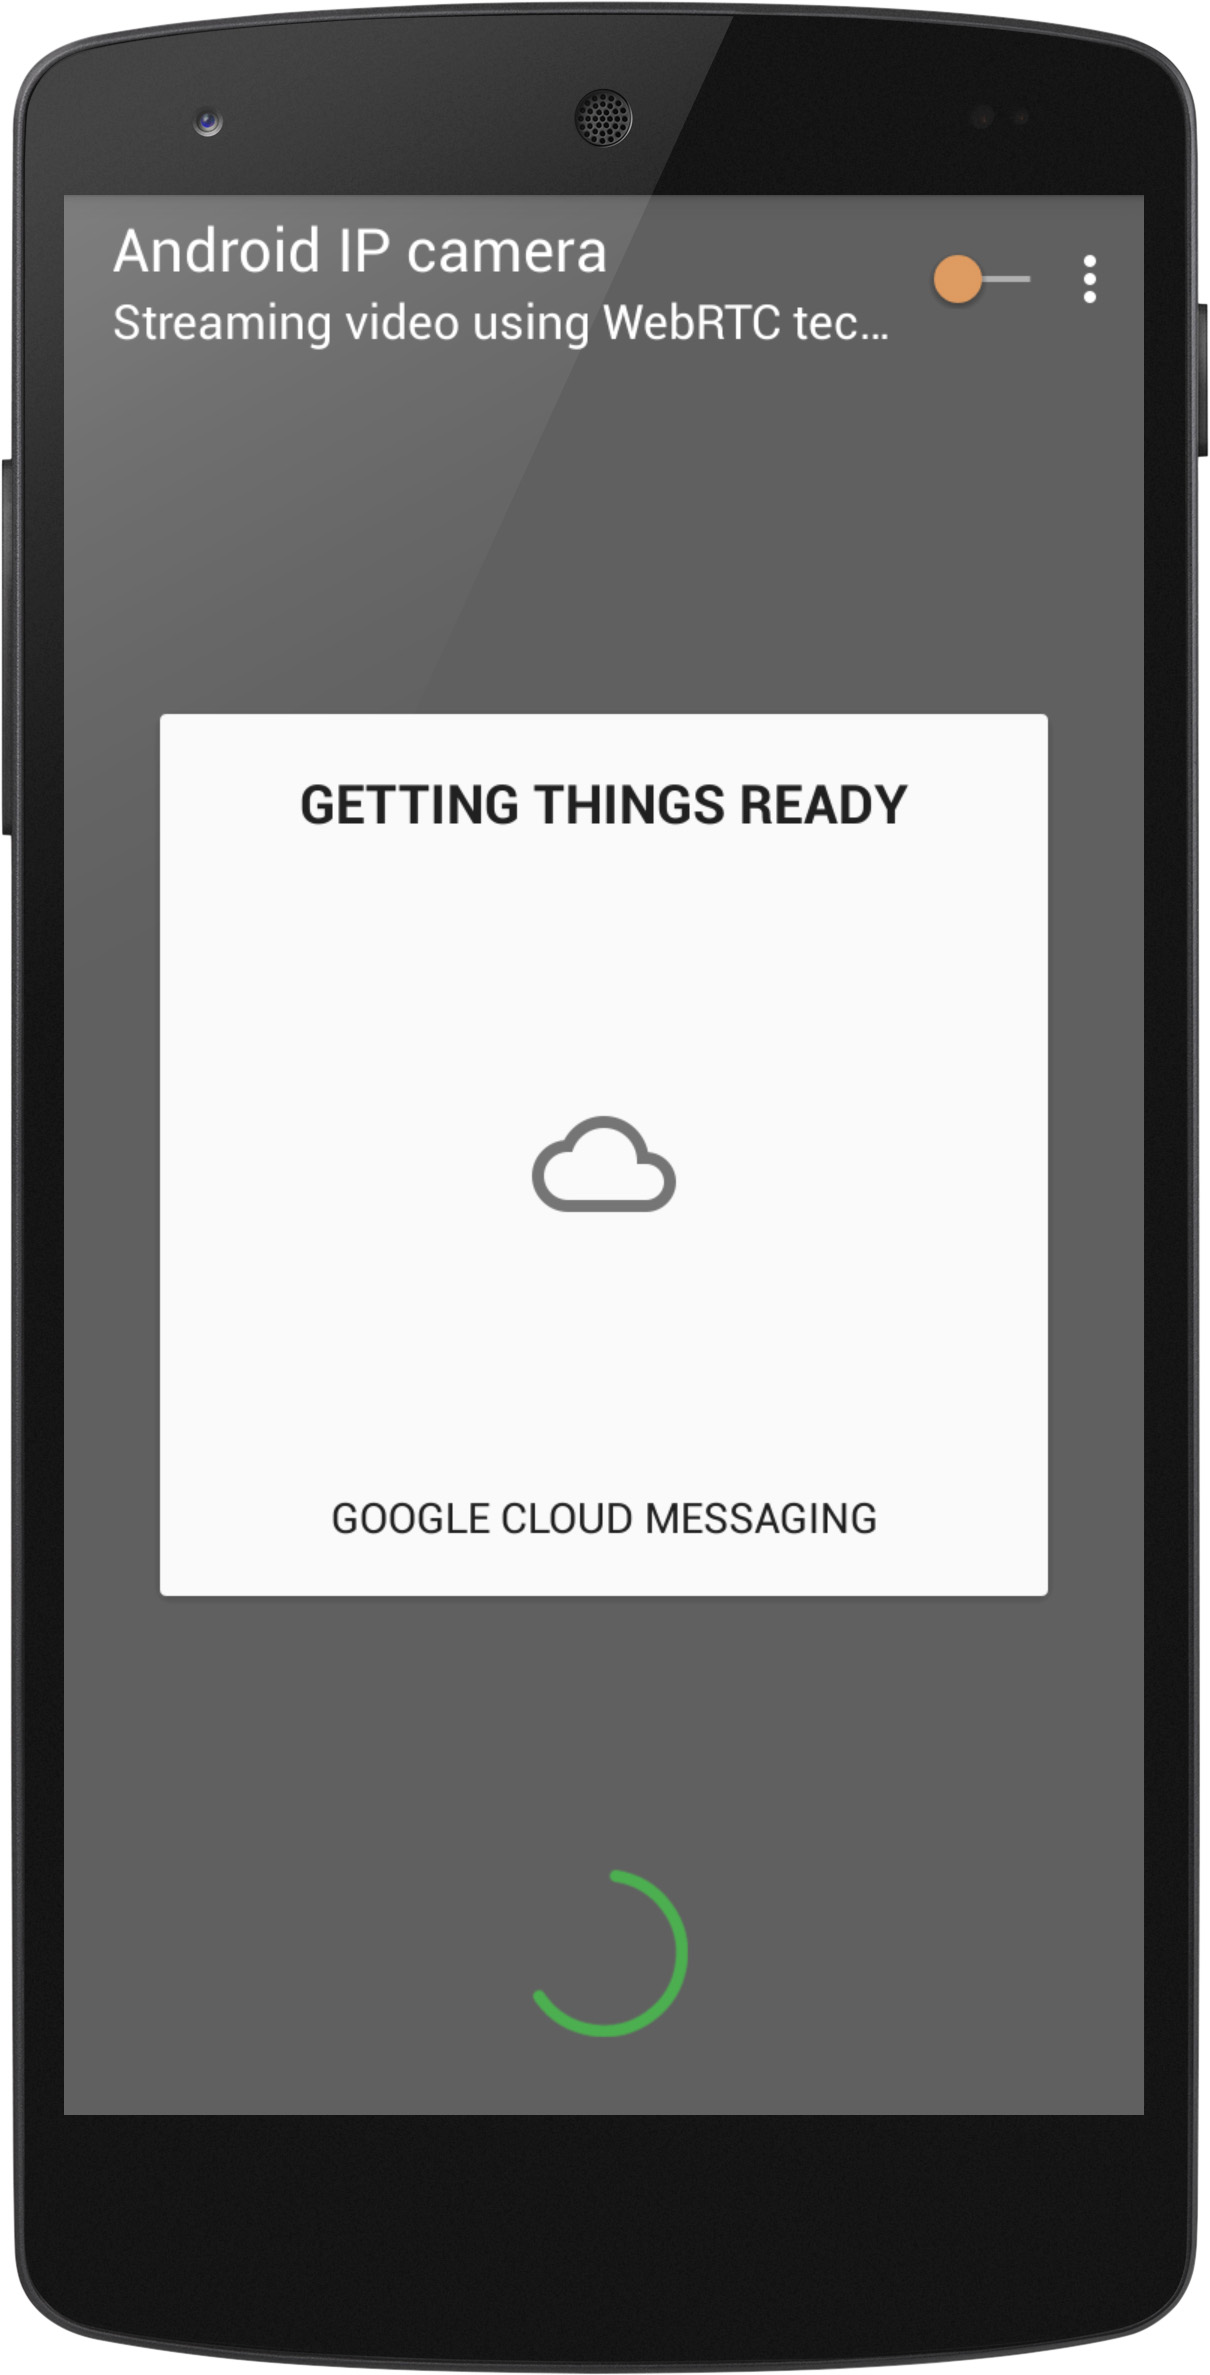
\includegraphics[width=0.24\linewidth]{fig/screenshots/screenshot1_framed.jpg}
	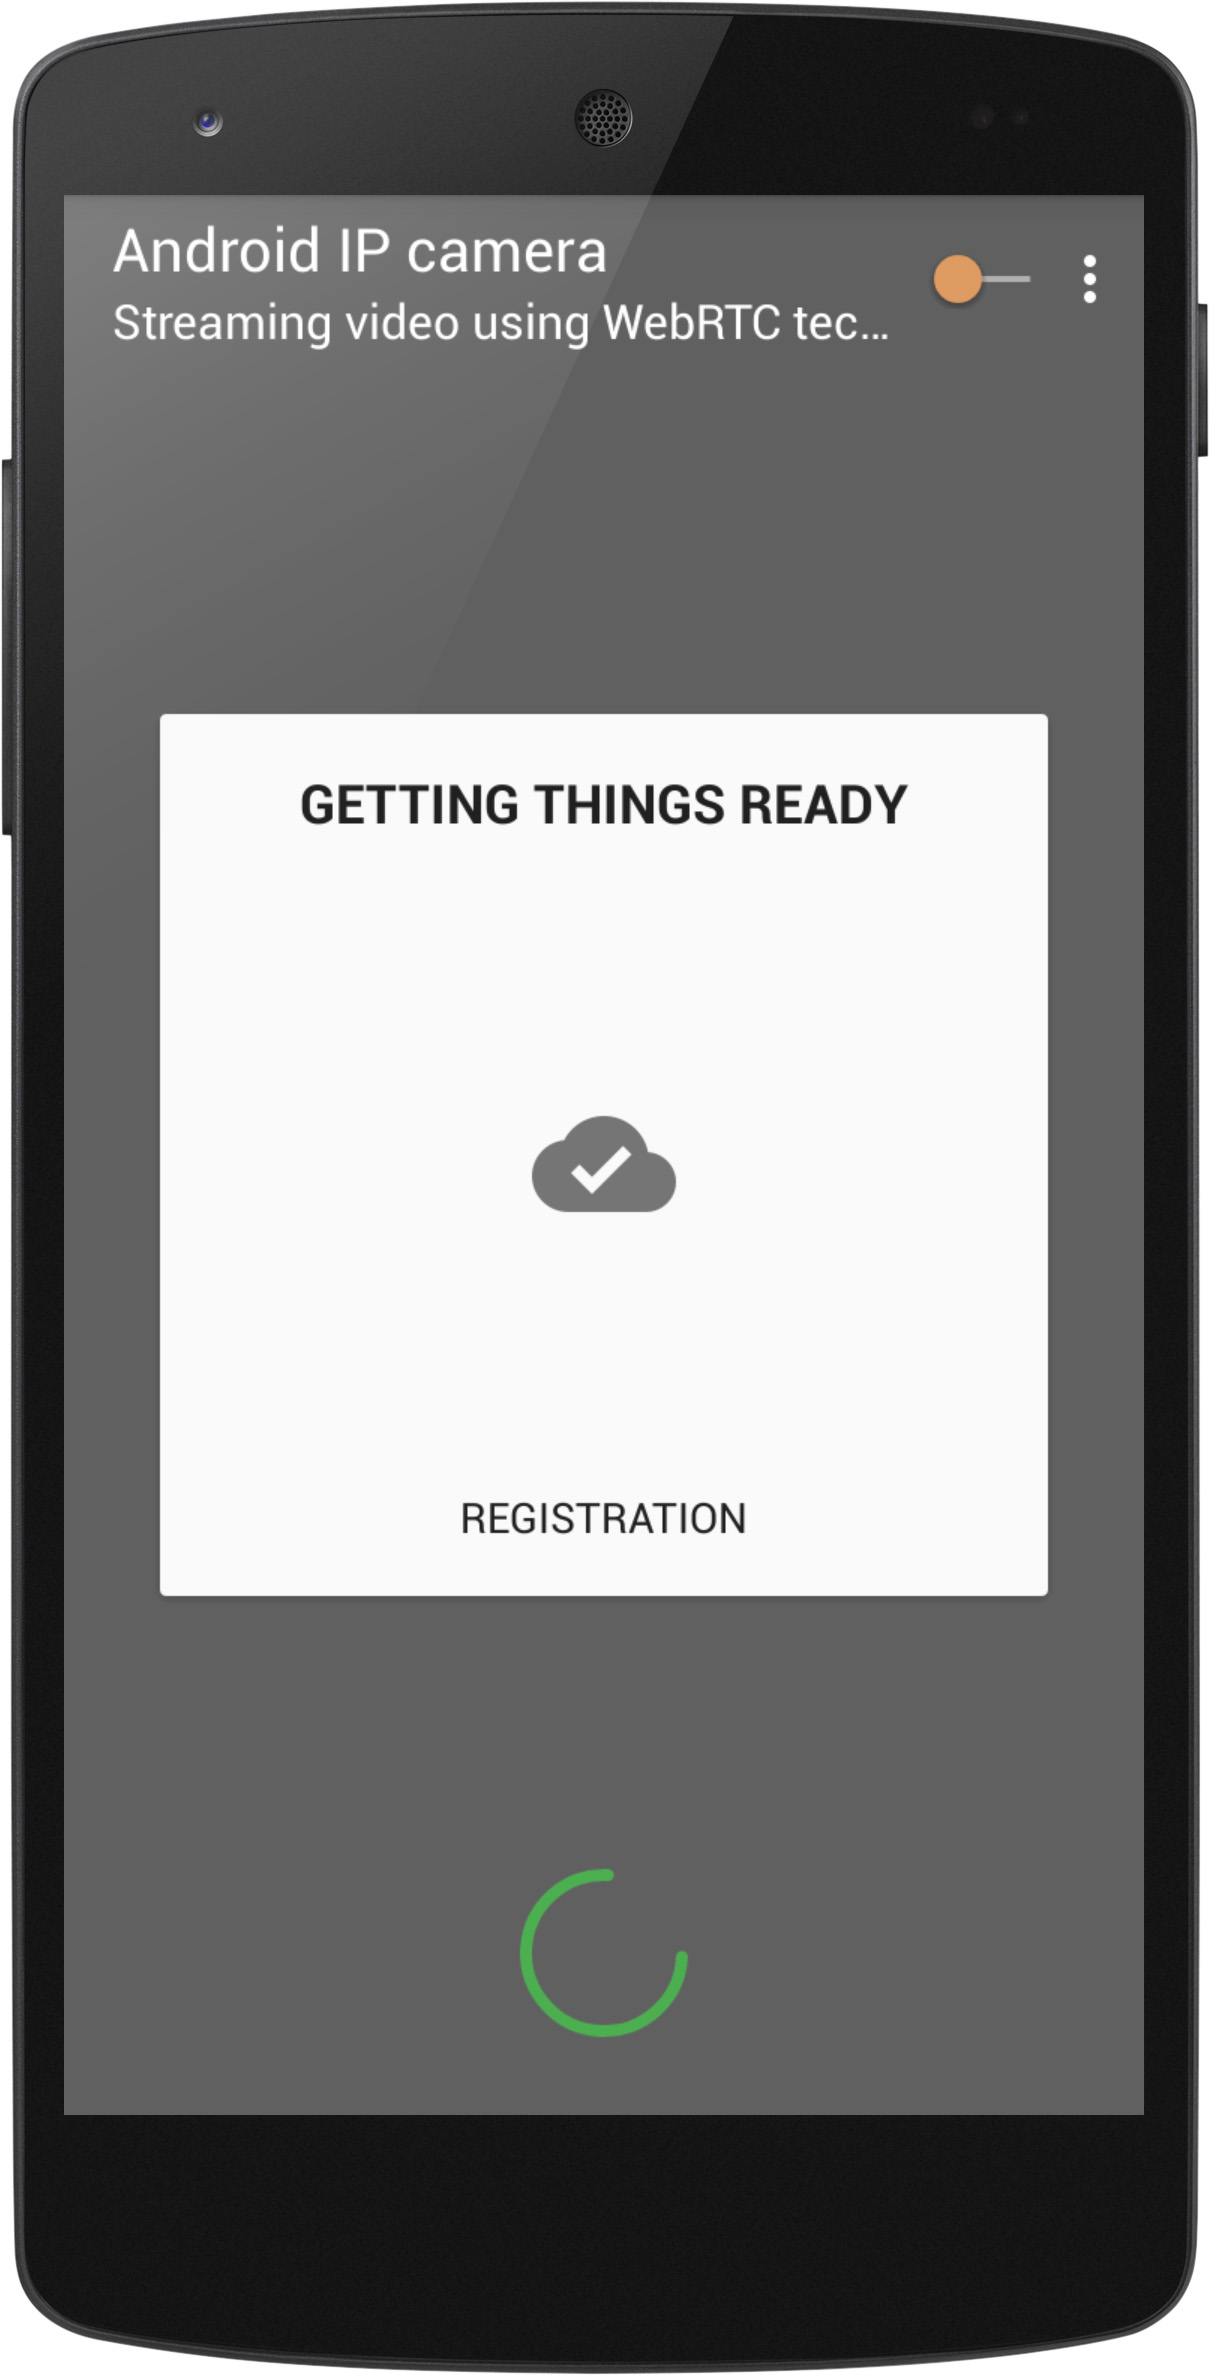
\includegraphics[width=0.24\linewidth]{fig/screenshots/screenshot2_framed.jpg}
	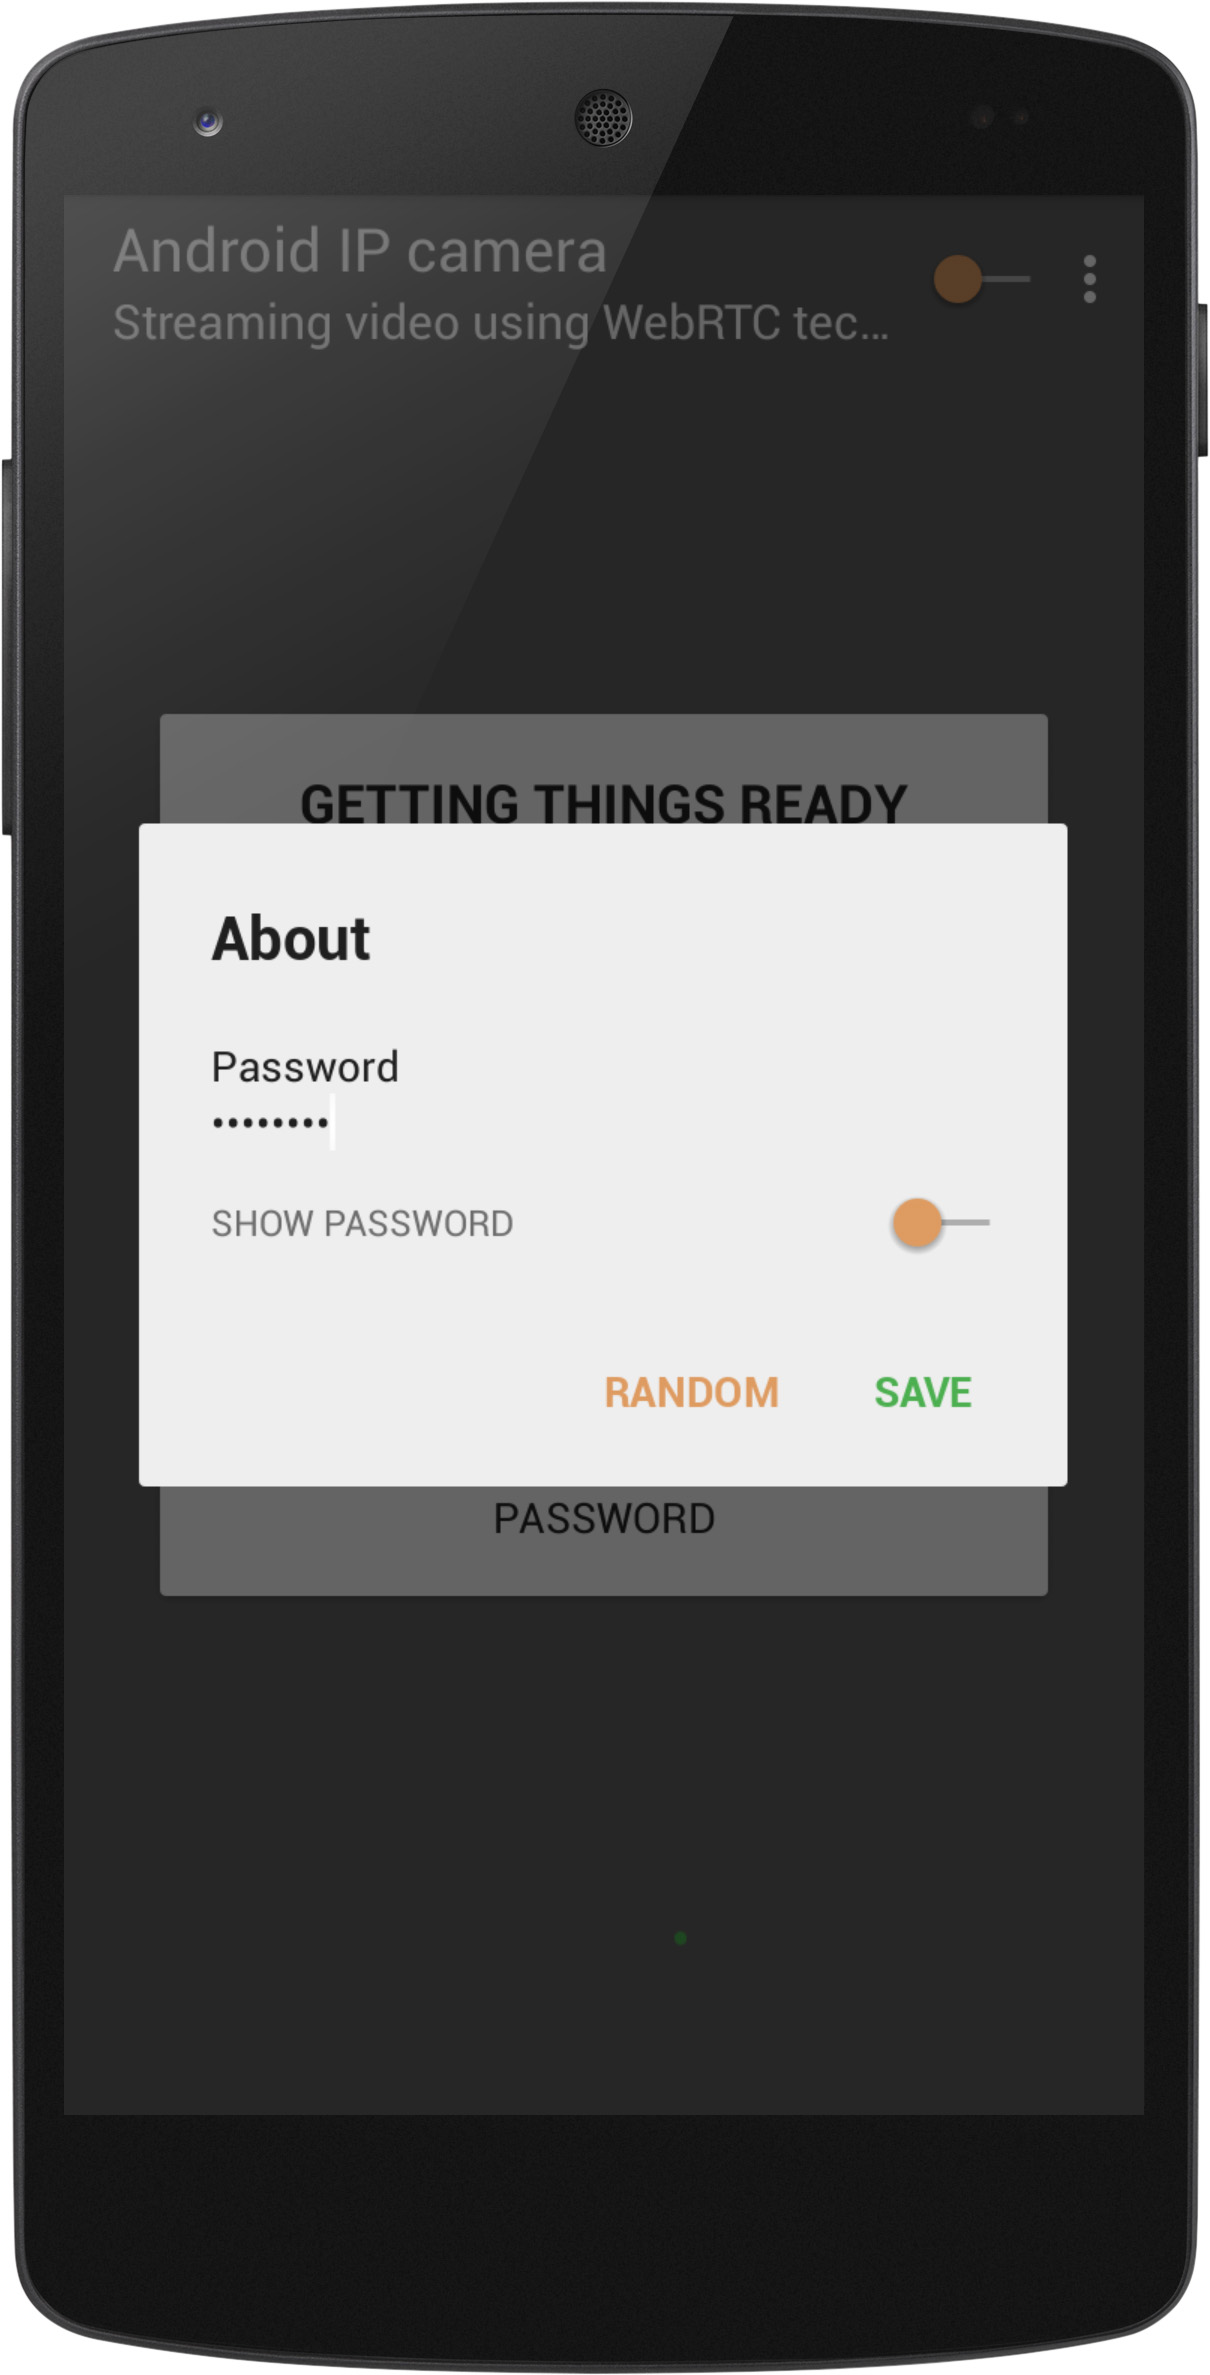
\includegraphics[width=0.24\linewidth]{fig/screenshots/screenshot3_framed.jpg}
	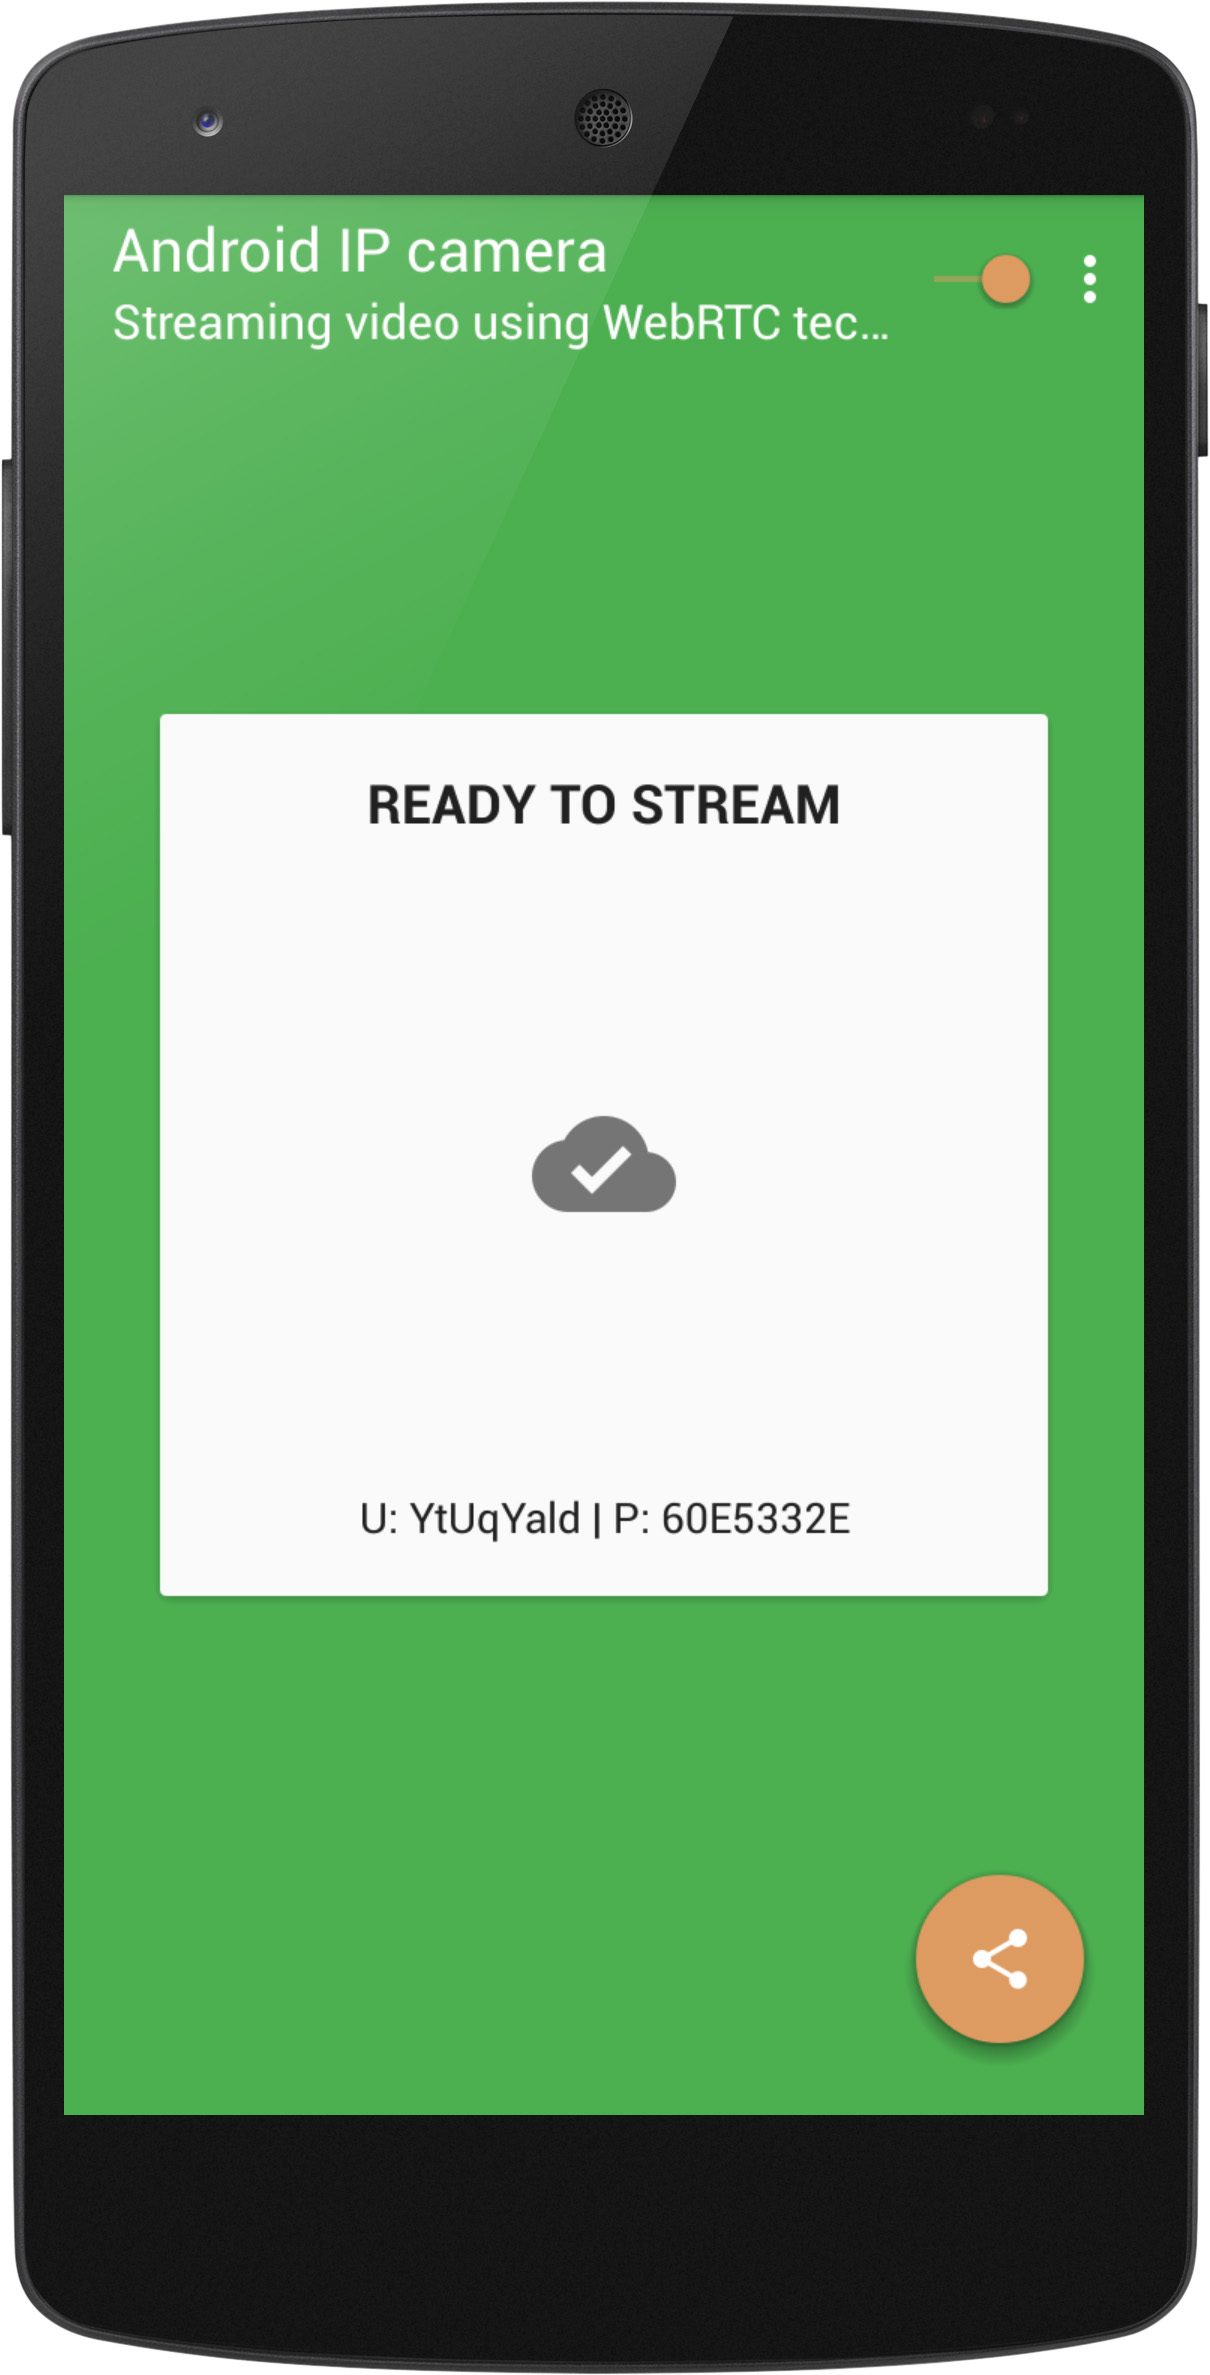
\includegraphics[width=0.24\linewidth]{fig/screenshots/screenshot4_framed.jpg}
	\caption{Screenshots of application's registration process. From left: GCM registration, registration to application server, password setting and ready to stream screen.}
	\label{fig:impl-screenshots1}
\end{figure}


After the registration is completed the user has the possibility to enable the incoming GCM requests for the streaming. This is done with the switch located in Toolbar at the top of each screen, see the last image in figure \ref{fig:impl-screenshots1}. The state of the application is indicated in Card Fragment and also with the background colour which is indicating the state for the first sight.

\begin{figure}[H]
	\centering
	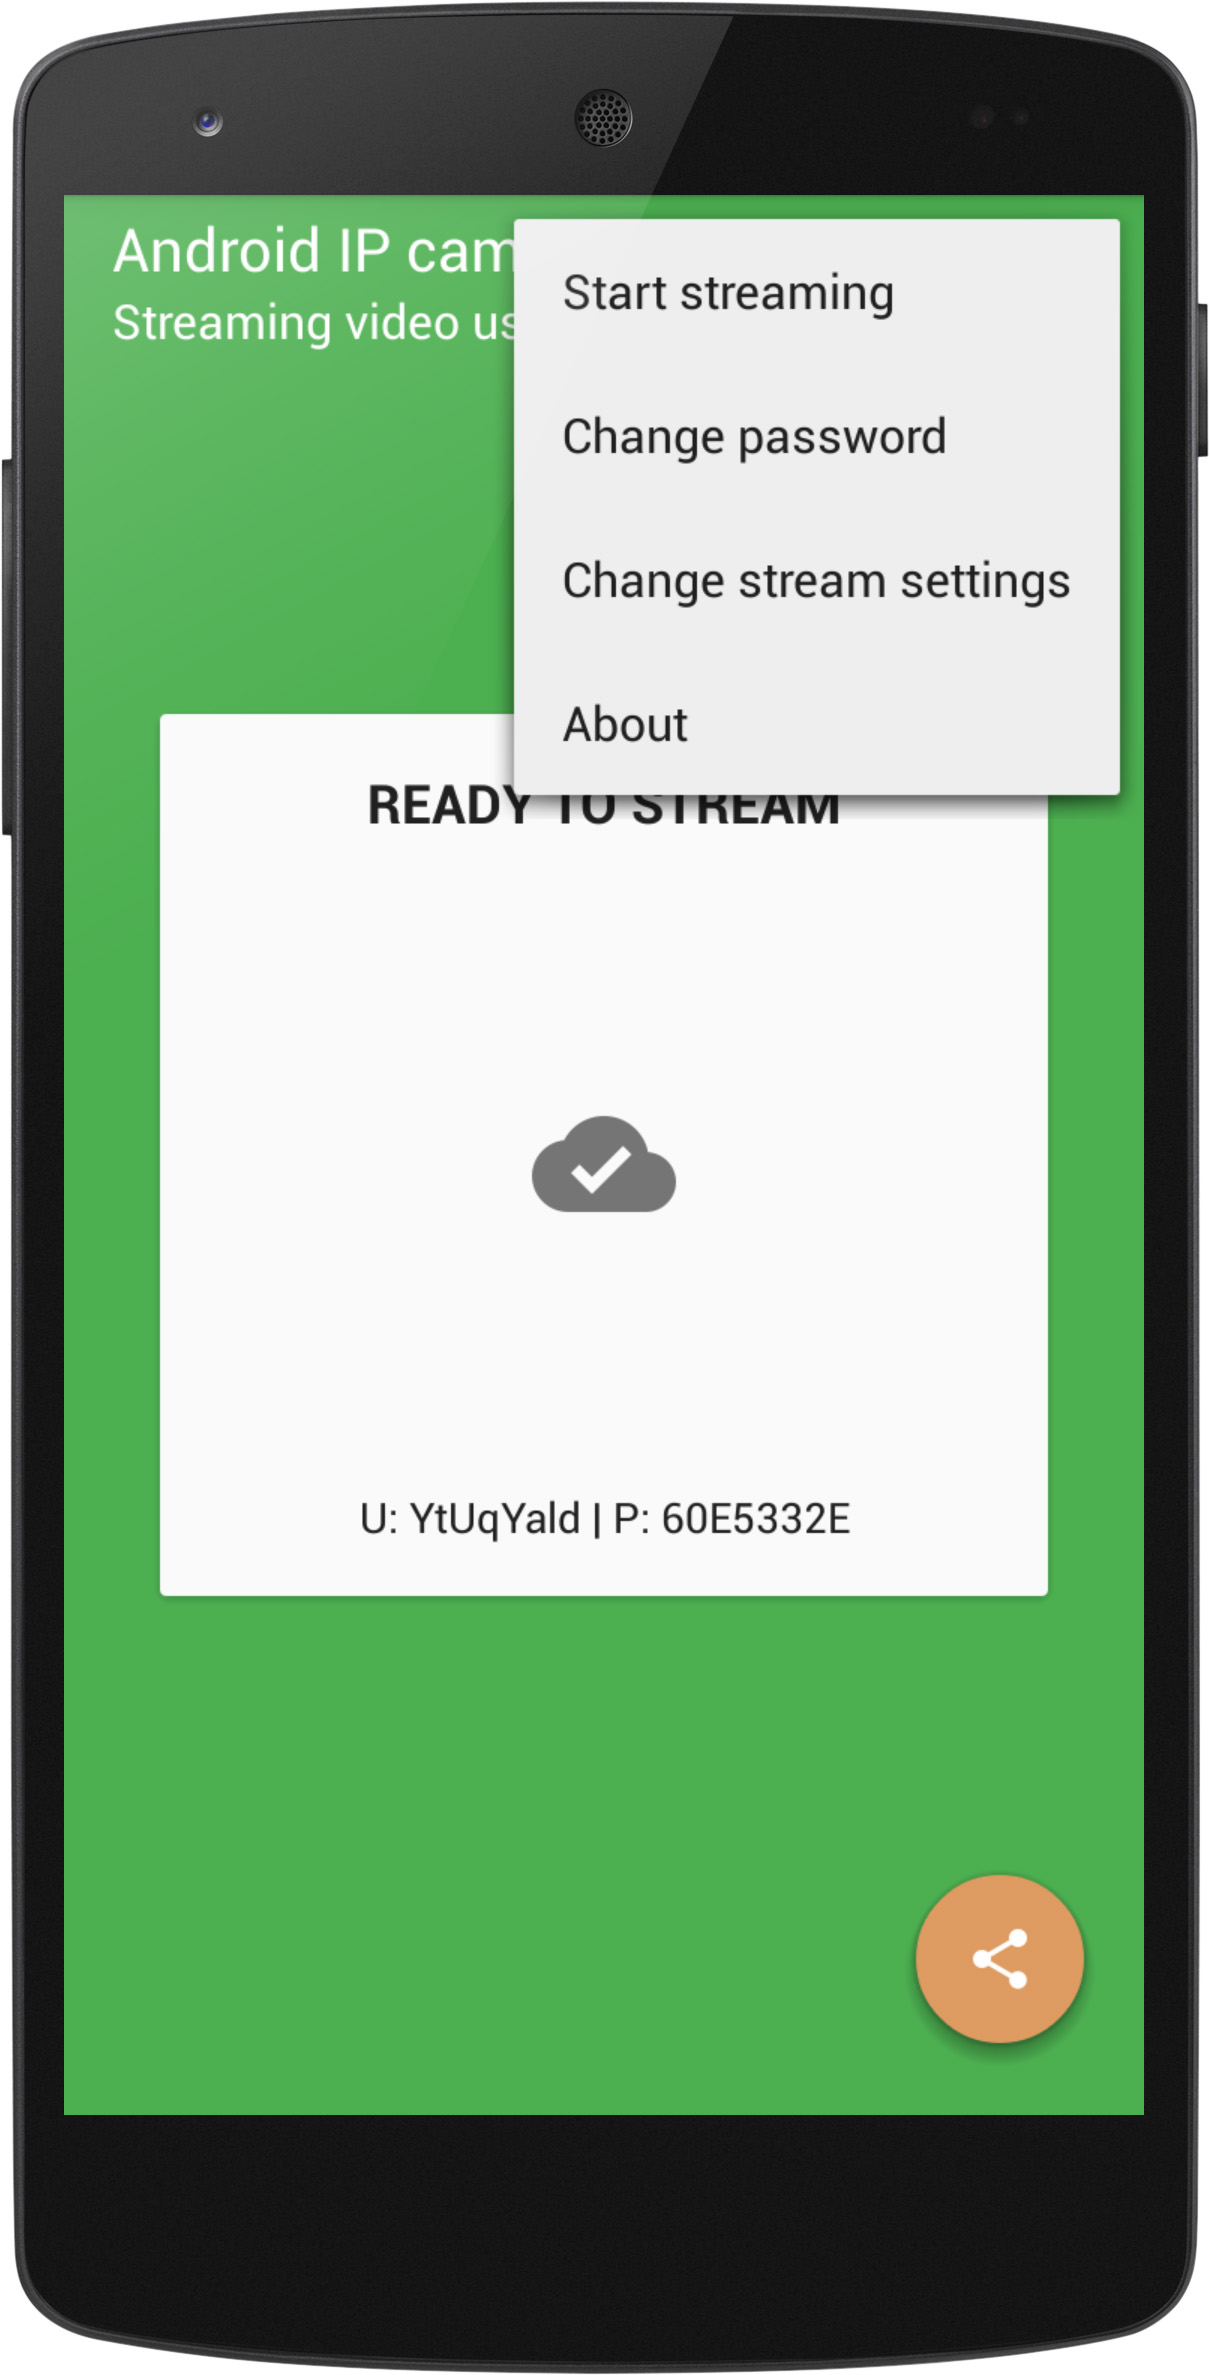
\includegraphics[width=0.24\linewidth]{fig/screenshots/screenshot5_framed.jpg}
	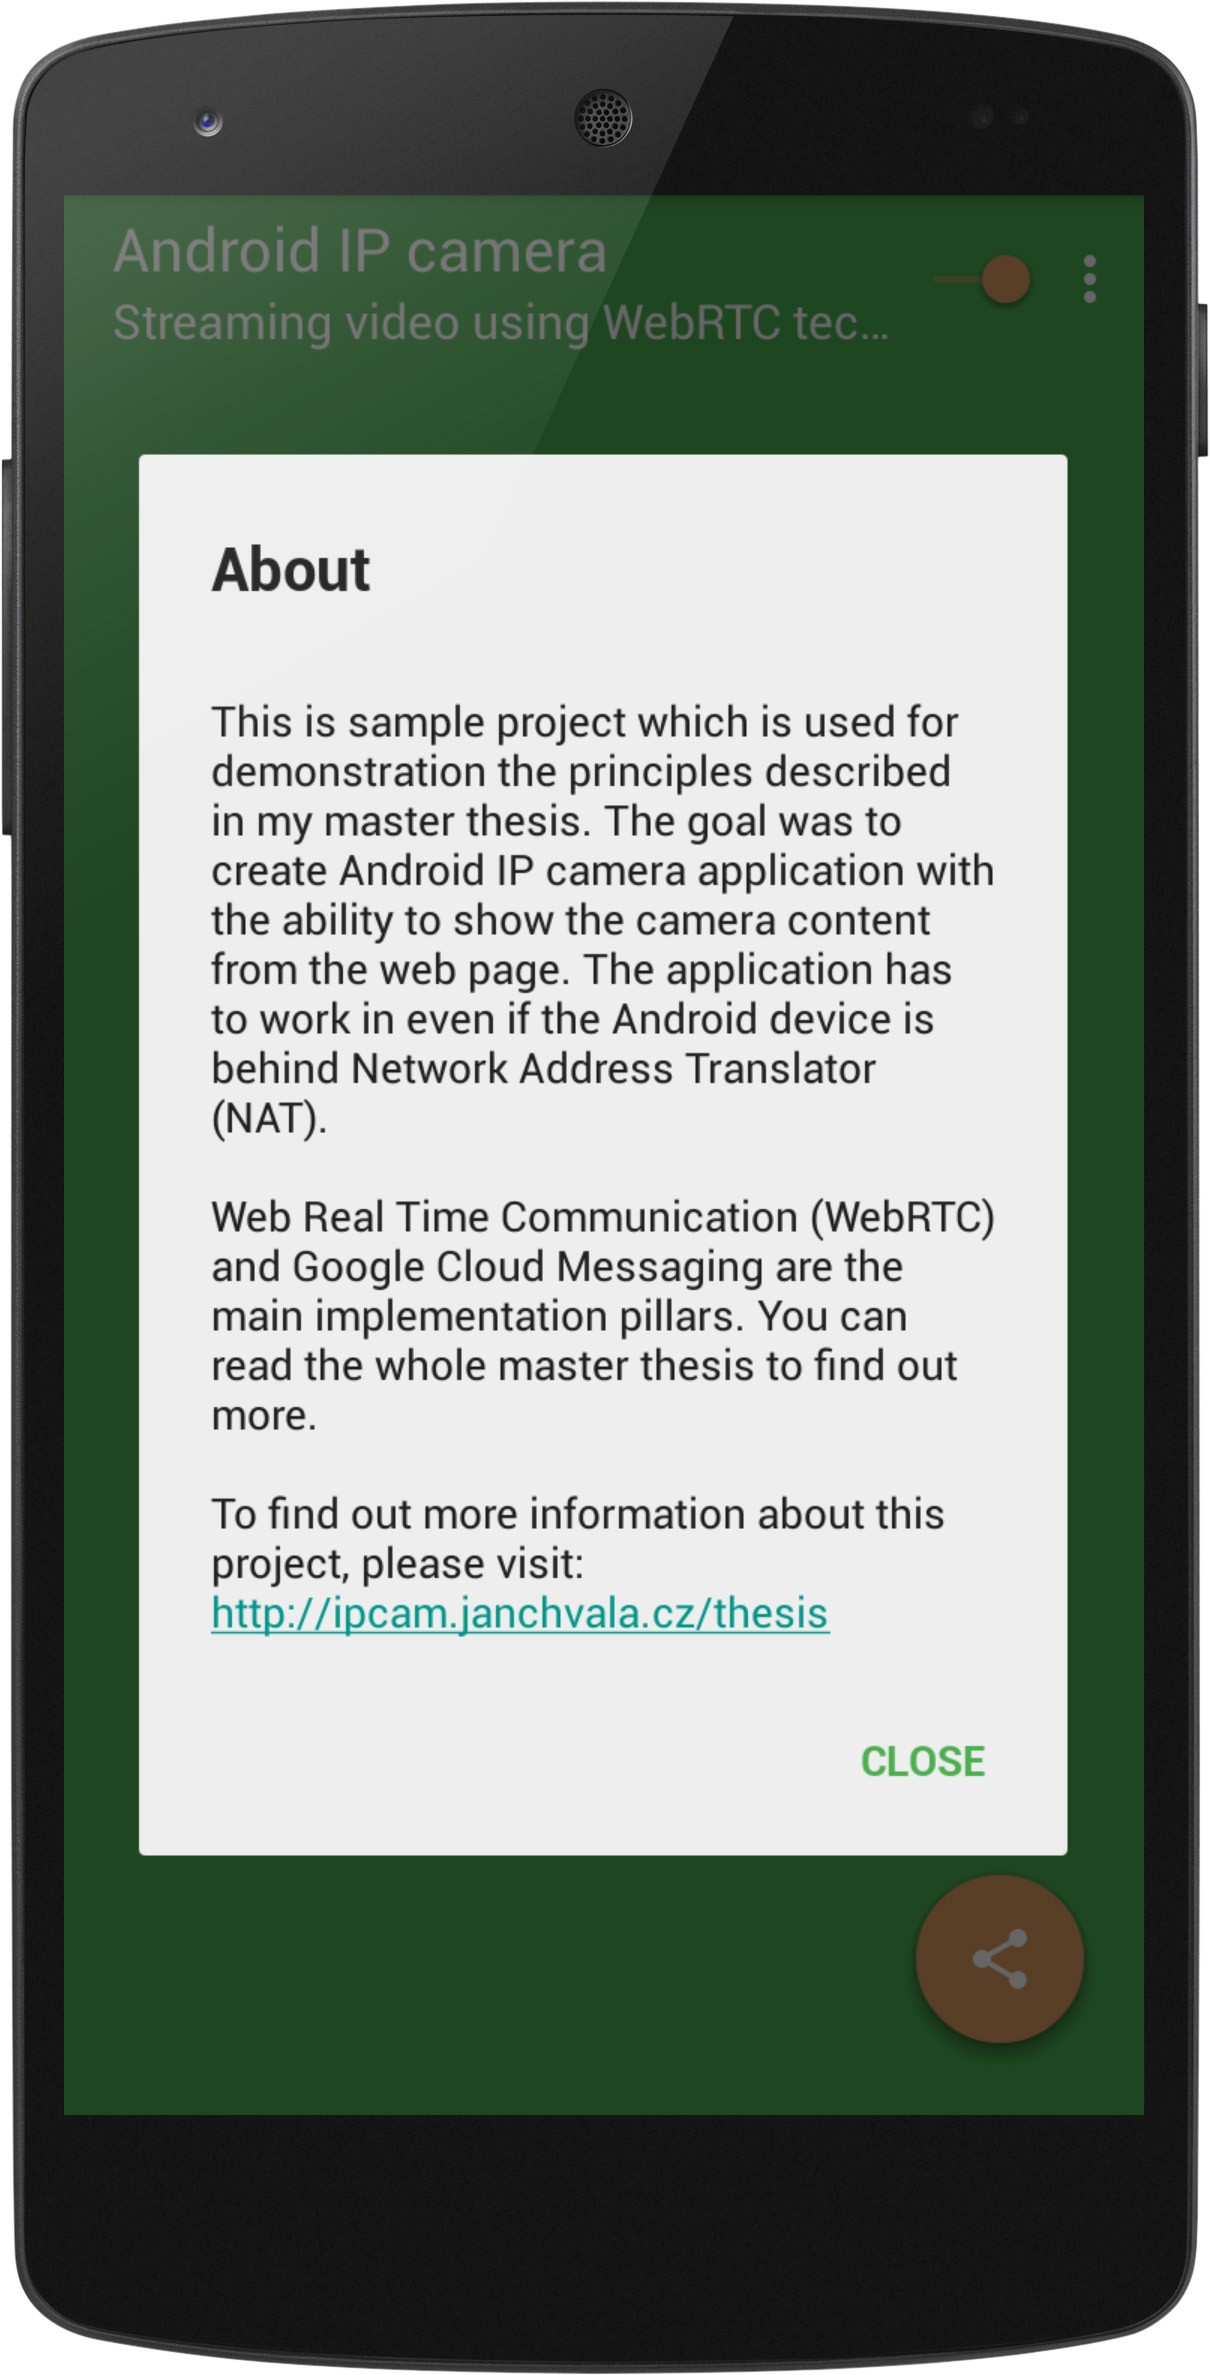
\includegraphics[width=0.24\linewidth]{fig/screenshots/screenshot6_framed.jpg}
	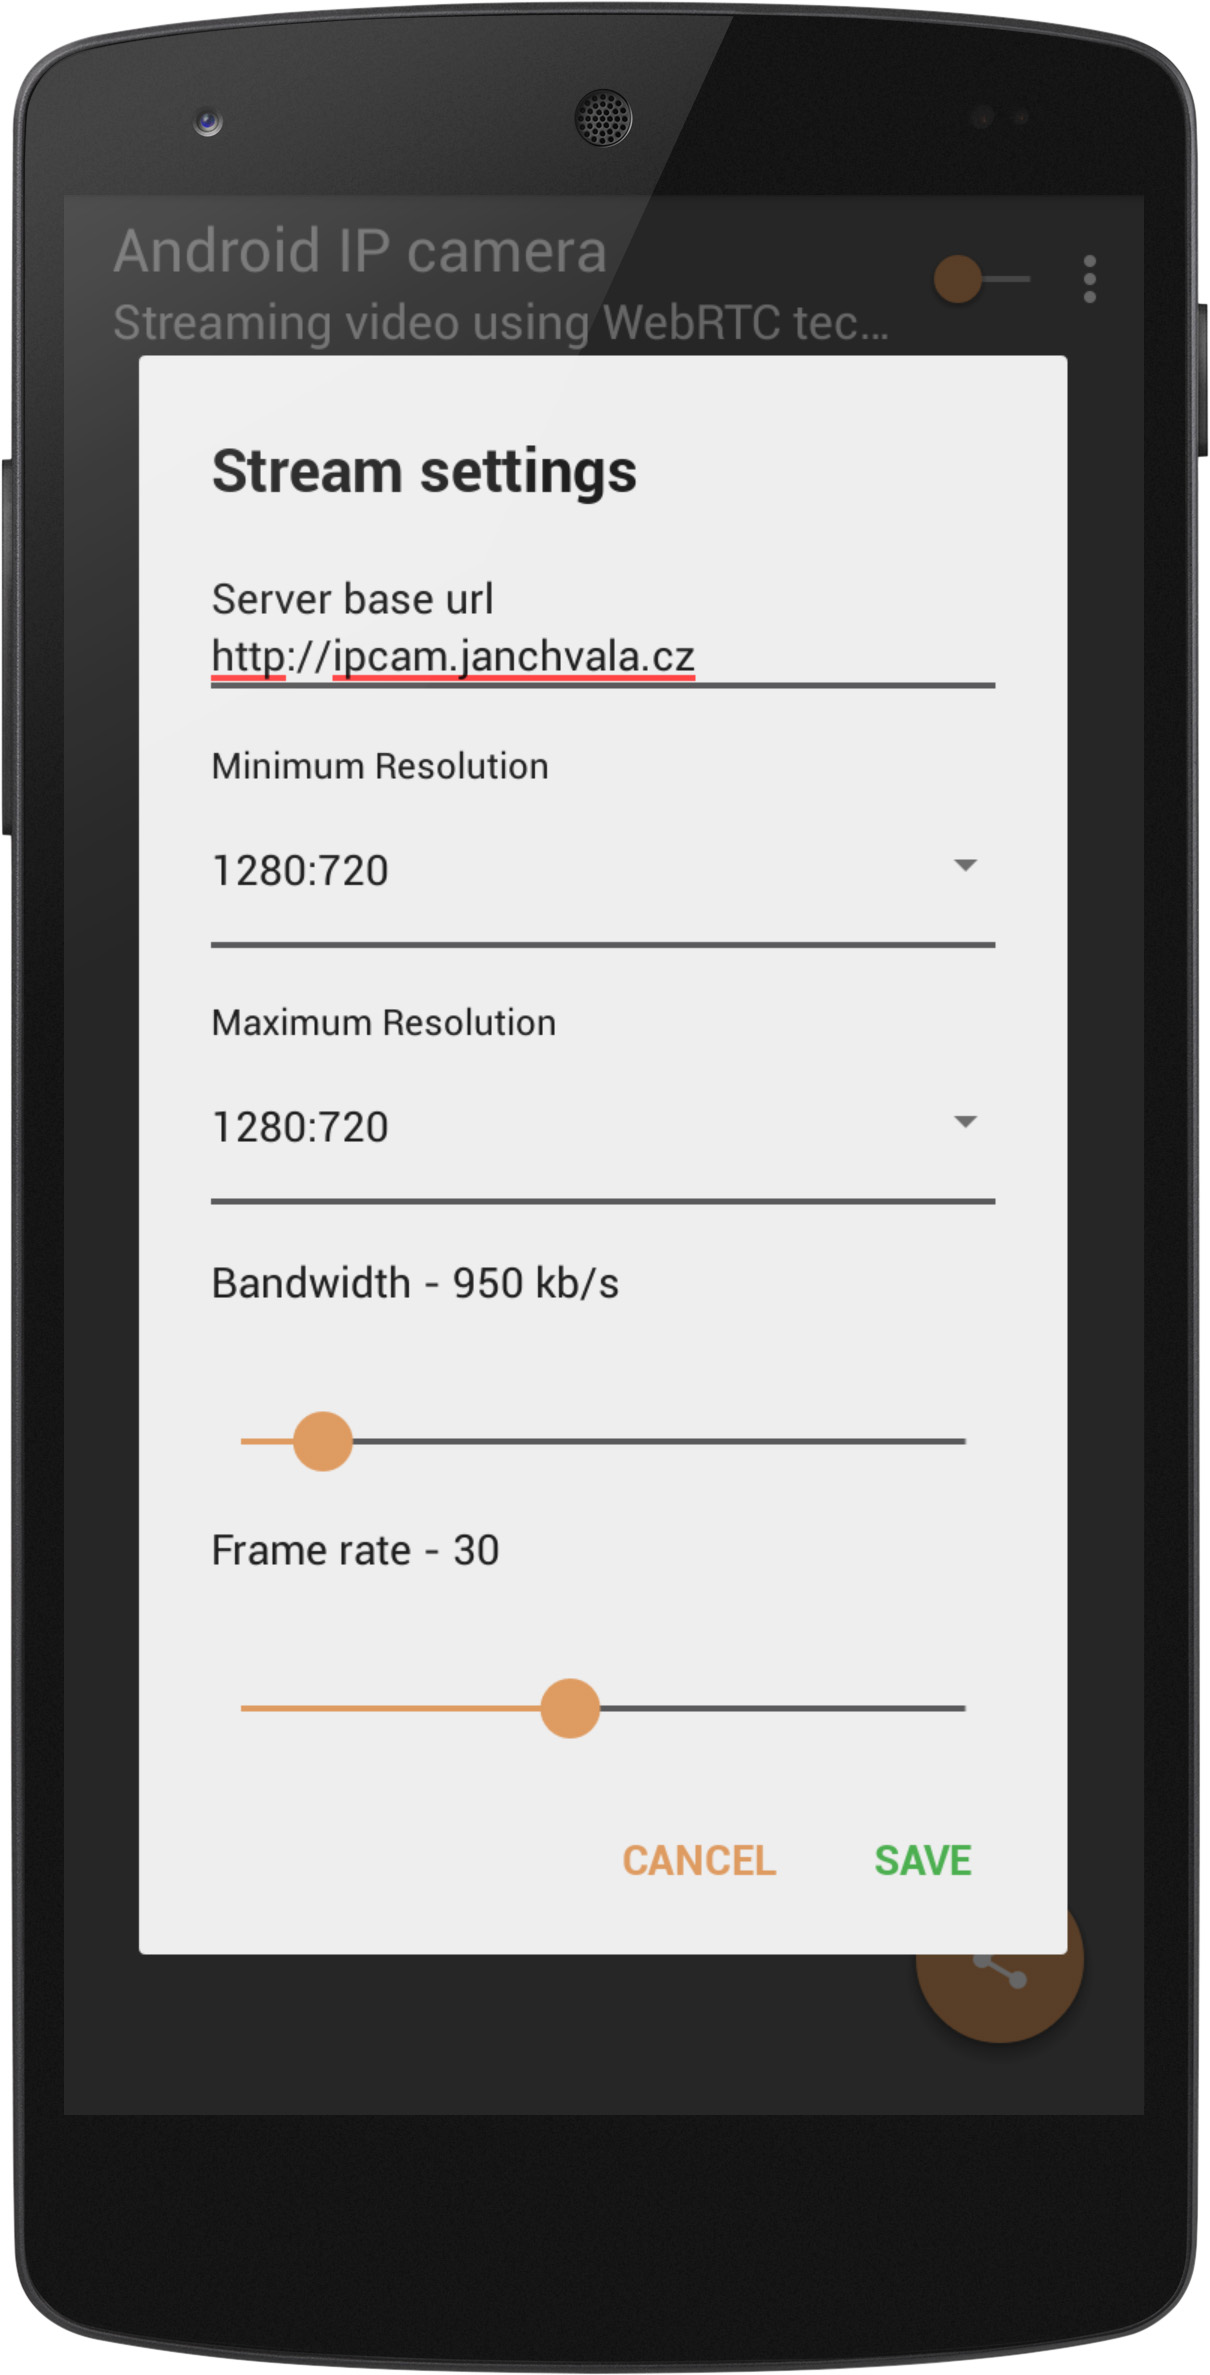
\includegraphics[width=0.24\linewidth]{fig/screenshots/screenshot7_framed.jpg}
	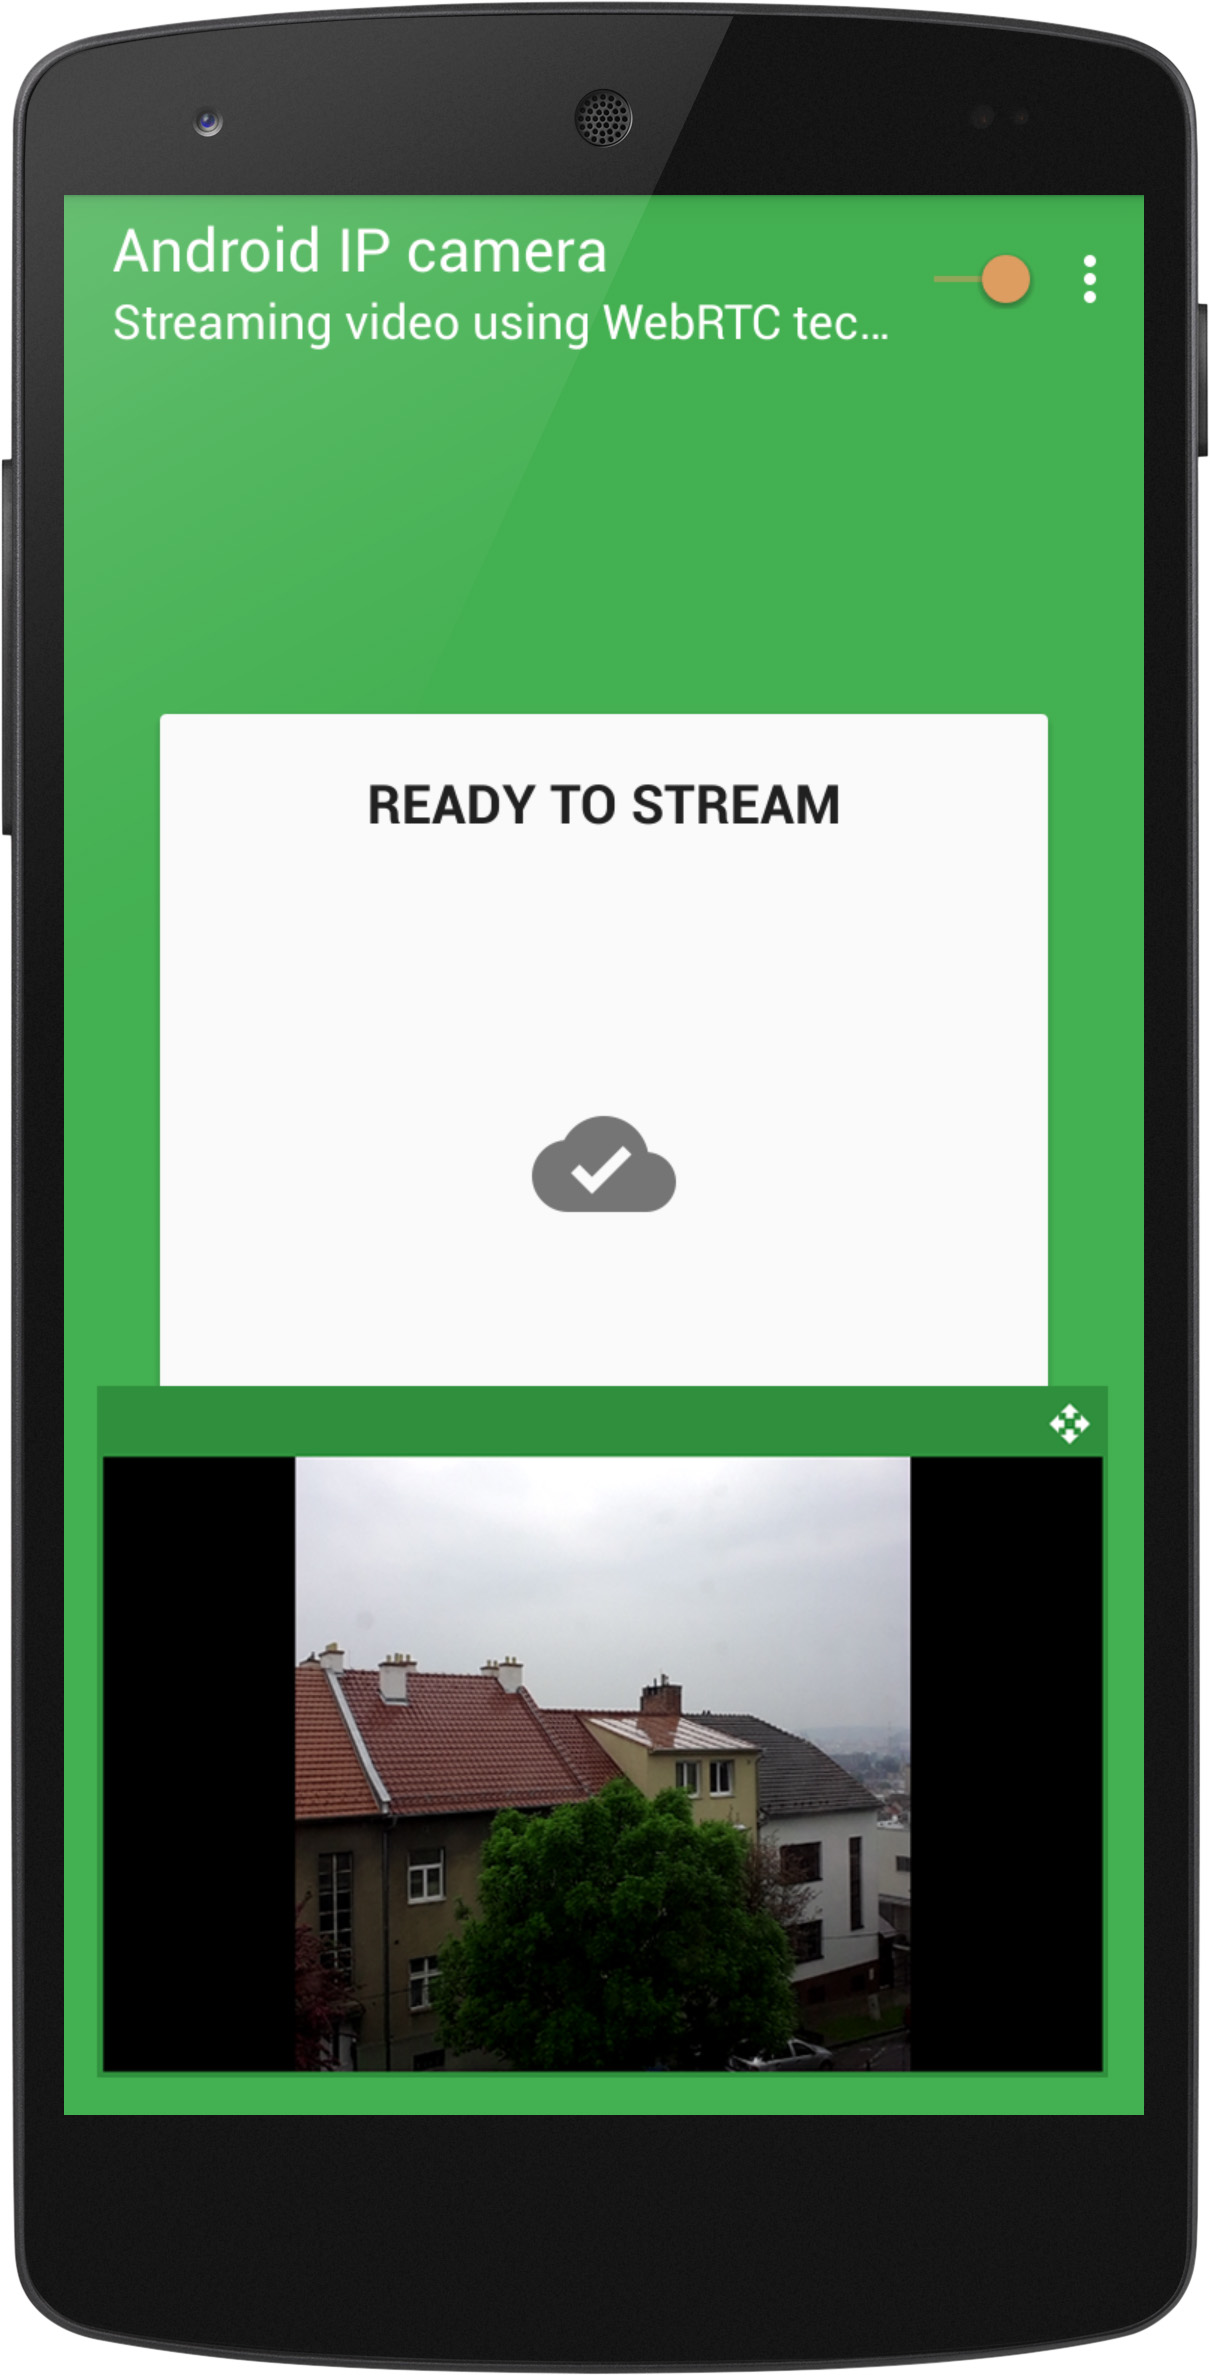
\includegraphics[width=0.24\linewidth]{fig/screenshots/screenshot8_framed.jpg}
	\caption{Screenshots of application during registration process and streaming. Last screenshot also shows streaming notification.}
	\label{fig:impl-screenshots2}
\end{figure}

\newpage
The application provides some actions for the user. Quick action to share the stream URL is accessible from FAB\footnote{Floating Action Button -- circular button introduced in Material design guidelines\\ \url{http://www.google.com/design/spec/components/buttons-floating-action-button.html}} in the left bottom corner of the screen while the others are located in the overflow menu\footnote{Overflow menu is indicated with three vertically aligned dots above each other.}. With these actions the user can easily change the password the same way he initialized it, change stream parameters, start the streaming explicitly or show simple information about the application.

It is also possible to change the server base url which is useful if application url changes. Server registration is reset and new request for streaming code is triggered by changing this option.

Last screen shot shows the notification and also tablet layout user interface. The user has the possibility to stop the streaming or share the streaming URL via notification's buttons. The notification is shown in figure \ref{fig:impl-screenshots3} but it is shown only on Android Lollipop when streaming with native WebView component.

\insertImgHere[1.0]{screenshots/tablet-notification.jpg}{Screenshots of  notification during streaming. Tablet UI.}{fig:impl-screenshots3}

\newpage
\subsection{Handling Google Cloud Messages and streaming}
Google Cloud Messages are processed in three steps in three different parts of the application. The message is invoked the stream is requested by the streaming page \ref{subsec:streaming-page}.

\subsubsection{Receiving messages using BroadcastReceiver}
\textit{GcmBroadcastReceiver} extends \textit{WakefulBroadcastReceiver} which is used to make device awake while receiving messages. It is registered in \textit{AndroidManifest} (\ref{android:manifest}) and it is the first part of the application which is invoked when GCM message is received.

\begin{lstlisting}
@Override
public void onReceive(Context c, Intent intent) {
  // specify that GcmIntentService will handle the intent
  String serviceName = GcmIntentService_.class.getName();
  ComponentName cName = 
    new ComponentName(c.getPackageName(), serviceName); 
  intent.setComponent(cName);

  // Start the service and keep device awake
  startWakefulService(c, intent);

  // set the result of this receive as success
  setResultCode(Activity.RESULT_OK);
}
\end{lstlisting}

\subsubsection{Processing messages using IntentService}
After receiving the message in \textit{BroadcastReceiver} the message is resent to \textit{GcmIntentService} that takes proper action for the message. If it is a real GCM message (not error or deleted event) then the stream is started.
\begin{lstlisting}
@Override
protected void onHandleIntent(Intent intent) {
  Bundle extras = intent.getExtras();
  if (!extras.isEmpty()) { // Initialize GCM
    GoogleCloudMessaging gcm = GoogleCloudMessaging.getInstance(this);

    // getting the message type
    String messageType = gcm.getMessageType(intent);
    // If this is a regular message then start stream
    String mType = GoogleCloudMessaging.MESSAGE_TYPE_MESSAGE;

    if (mType.equals(messageType)) {
      Class wClass = IpCamPreviewWindow_.class;
      Intent i = StandOutWindow.getShowIntent(this,wClass,0);
      startService(i);
    }
  }

  // Releasing the wake lock
  GcmBroadcastReceiver.completeWakefulIntent(intent);
}
\end{lstlisting}

\subsubsection{Starting the stream Service}
Stream is started using \textit{IpCamPreviewWindow\footnote{This window is service with specific UI elements floating above other windows in the system. This is made possible by StandOut library: \url{https://github.com/sherpya/StandOut/}}}. This service creates new \textit{Window} object which can hold UI elements and it is inflated with \textit{WebView}. Then the \textit{WebView} loads streaming page from application server and \textit{WebRTC} takes care about the rest of the streaming. The code below shows the layout inflation and \textit{WebView} initial settings.

\begin{lstlisting}
@Override
public void createAndAttachView(int id, FrameLayout frame) {
  // create a new layout from body.xml
  LayoutInflater inflater = (LayoutInflater) getSystemService(LAYOUT_INFLATER_SERVICE);
  inflater.inflate(R.layout.ipcam_window_layout, frame, true);

  wv = (WebView) frame.findViewById(R.id.web_view_id);
  setupWebView(wv);
}

/**
 * setup WebView JavaScript, ChromeClient and load stream page
 */
protected void setupWebView(WebView wv) {
  WebSettings webSettings = wv.getSettings();
  webSettings.setJavaScriptEnabled(true);
  ...
  wv.setWebChromeClient(new WebChromeClient() {
    @Override
    public void onPermissionRequest(final PermissionRequest request) {
      // handling WebRTC permission request
      dispatchPermissionRequest(request);
    }
  });
  wv.loadUrl(IntentHelpers.getStreamUrl(ipCamPreferences));
}
\end{lstlisting}

\noindent
To see how GCM is registered, see section \ref{ssec:gcm-register}.






%\section{Request to start the stream remotely}
%\blind{1}

%\subsection{Use case}
%\blind{1}
%\todoImg
%\blind{1}

%\subsection{Starting the stream -- client}
%\blind{1}

%\insertImg[0.7]{placeholder.pdf}{Communication when the stream is requested.}{fig:impl-stream-page}

%\subsection{Requesting the playback -- server}
%\blind{1}
%\todoImg
%\blind{1}




\newpage
\section{Security and authentication in demo application}
The authentication and security is not crucial for demonstration of WebRTC technology but it is not desirable to allow anybody to see private streaming.

The application allows to protect device stream with a password which is set up during application first launch on Android device (it can be changed later on). This password is checked on every request from a participant to join created streaming session. The request is then accepted or rejected based on password equality.

\begin{lstlisting}
// set up the password with JavaScript interface from Android
var password = Android.getPassword();

// participant requests access to session
connection.onRequest = function(e) {
  // check if the passwords equal
  if (e.extra.password !== password){
    // the passwords do not match - reject access
    connection.reject(e);
  } else { // accept the request
    connection.accept(e);
  }
};
\end{lstlisting}


There is no protection for the server REST API so anybody who can catch the device code can simply start the stream on the device. We would have to implement user management and registration on the server side to be able to protect it which is out of scope of this thesis. With that in mind the demo application is not intended to be a ready production because of the lack of server REST API protection.

\section{The choice of WebRTC library}
There were more options to choose from when deciding which library to use when working with WebRTC. A few developers try to use the WebRTC and thus they build libraries on top of this edge technology. This section will shortly describe considered libraries and the reasons why they were chosen or not.

\subsection{PeerJS}
The first option found was PeerJS\footnote{PeerJS homepage:\url{http://peerjs.com/}} library. This library is very simple to use and from my point of view it is the easiest to work with. It has very simple API and it also provides the ability to use free \textit{PeerServer} which is responsible for the signalling process.

The main problem is that this library does not support one way video streaming. This is crucial for the resultant application because it is not desirable to request permissions from the user who only wants to play the video stream.

Another problem for me concerning this library is that it seems to be stuck in development. Their master branch on GitHub repository is four months old and it does not seem to be progressing.

\subsection{RTCMultiConnection v2}
Another solution that was the one actually used in the resultant application was the RTCMulticonnection\footnote{RTCMultiConnection homepage: \url{http://www.rtcmulticonnection.org/}} in its version 2.2.2. This library is well documented and allows a lot of customizations. There are also many good examples of working with this library.

The main reason for using this library is that it supports one--way multimedia streaming. This allows to request permission only from the streaming device. It also reduces the data transmission because the session does not contain any empty streams which could affect the bandwidth.

Another good reason is that Muaz Khan (The author of this library) has made it open sourced and he is very actively working on it.

\subsection{RTCMultiConnection v3 beta}
A new version of previously mentioned library was published on 1st April. I was trying to switch the resultant application to use this new version of the RTCMultiConnection library, which provides some more functionality such as build in room protection by password.

It also comes with signalling server build on top of Node.js which is the technology used for the application server. But it is still in beta and there were problems with the signalling process. The problems were making the established connection to fall apart after a couple of seconds of successful stream transmission.

There is a lot of going on around this library and we can be looking forward to seeing its improvements in the near future. I would recommend taking a look at this library for those interested in working with WebRTC.\\

  %=========================================================================
% 
\chapter{Testing and flaws}
\label{chap:chapter6}
This chapter focuses on the testing of the resultant application in real conditions. In the first part of this section there are measurements of delays and connectivity establishment. The second part points out some of the problems, which occurred during the development process.


\section{Measuring streaming delays and stability testing}
Important aspects of real--time streaming are delays. Everything takes time. Loading the page inside the browser, starting the device with GCM, acquiring local media, Peer Connection establishment and media transfer. These delays make the difference between a usable and unusable solution.

The resultant system was created to work in most cases even when the device is hidden behind NAT and to stream data only when it is needed. All the technologies that make this possible are against the speed of the process from the point where the stream is requested to the point where it is actually shown to the user.


\subsection{Delays}
 The streaming application is expected to be running on local wi--fi network and to be placed stationary. In this way the streaming was tested. The requests on the other hand may be done from different networks with different capabilities. Because of that the testing requests were made from three different networks: Wi-fi, 3G and mocked 2G network\footnote{The 2G network was mocked by disabling 3G connectivity on mobile device.}. For each connectivity except 2G newrok\footnote{Testing of requests from 2G networks was very unstable. The connection could be established for the lowest possible streaming quality only for three times out of thirty and they were not stable. All of them broke after a couple of seconds of streaming. Therefore using the resultant application on 2G networks is not recommended.} there was one hundred established streams. Arithmetic mean was taken as the result for each measured value.\\

\noindent
All the streaming was done for the best video settings:\vspace{-0.5em}
\begin{itemize}
	\item \textbf{resolution} - $ 1980\times1020 $px
	\item \textbf{frame rate} - 30 frames per second
	\item \textbf{bandwidth} - 8000kb/s
\end{itemize}

\newpage
\noindent
Measured delays are:\vspace{-0.5em}
\begin{itemize}
	\item \textbf{stream available} - From request to media element availability. Shown in table \ref{table:stream}.
	\item \textbf{initial video delay} - The delay between the time when stream is available and the time it is shown. Shown in table \ref{table:delay}.
	\item  \textbf{total time} - from starting the streaming page to showing the video. Shown in table \ref{table:total}.
\end{itemize}

\noindent
The testing was made in two modes:\vspace{-0.5em}
\begin{itemize}
	\item \textbf{already running} - The stream is running and the session was established. There is no need to send GCM requests.
	\item \textbf{not running} - The stream has to be started with GCM messages.
\end{itemize}

\begin{table}[H]
\caption{Tables showing average \textbf{stream available} for different networks. Top table for already running streaming and bottom for GCM started streaming.}
\begin{center}
\begin{tabular}{|l|l|l|l|}
\hline 
& min (ms) & max (ms) & arithmetic mean (ms) \\
\hline 
wi--fi & 1813 & 4354 & 2181 \\
\hline 
3G & 1901 & 4523 & 2390 \\
\hline 
2G & - & - & - \\
\hline
\end{tabular} 

\label{table:stream}
\vspace{1em}
\begin{tabular}{|l|l|l|l|}
\hline 
& min (ms) & max (ms) & arithmetic mean (ms) \\
\hline 
wi--fi & 6036 & 9129 & 6639 \\
\hline 
3G & 6656 & 9860 & 7183 \\
\hline 
2G & - & - & - \\
\hline
\end{tabular} 
\end{center}
\end{table}

\vspace{-2em}
\begin{table}[H]
\caption{Table showing average \textbf{initial video delay} for different networks. Top table for already running streaming and bottom for GCM started streaming.}
\begin{center}
\begin{tabular}{|l|l|l|l|}
\hline 
& min (ms) & max (ms) & arithmetic mean (ms) \\
\hline 
wi--fi & 510 & 7702 & 1538 \\
\hline 
3G & 922 & 3113 & 1948 \\
\hline 
2G & - & - & - \\
\hline
\end{tabular} 

\label{table:delay}
\vspace{1em}
\begin{tabular}{|l|l|l|l|}
\hline 
& min (ms) & max (ms) & arithmetic mean (ms) \\
\hline 
wi--fi & 464 & 1771 & 1214 \\
\hline 
3G & 1051 & 2196 & 1715 \\
\hline 
2G & - & - & - \\
\hline
\end{tabular} 
\end{center}
\end{table}

\vspace{-2em}
\begin{table}[H]
\caption{Table showing average \textbf{total time} for different networks. Top table for already running streaming and bottom for GCM started streaming.}
\begin{center}
\begin{tabular}{|l|l|l|l|}
\hline 
& min (ms) & max (ms) & arithmetic mean (ms) \\
\hline 
wi--fi & 2344 & 10823 & 4321 \\
\hline 
3G & 3083 & 6745 & 4838 \\
\hline 
2G & - & - & - \\
\hline
\end{tabular} 

\label{table:total}
\vspace{1em}
\begin{tabular}{|l|l|l|l|}
\hline 
& min (ms) & max (ms) & arithmetic mean (ms) \\
\hline 
wi--fi & 6808 & 10180 & 7854 \\
\hline 
3G & 7784 & 11260 & 8898 \\
\hline 
2G & - & - & - \\
\hline
\end{tabular} 
\end{center}
\end{table}

Both wi--fi and 3G are quite similar in the results. The stream object that is being placed into HTML DOM was accessible after two seconds when playing active stream and approximately seven seconds when it had to be started with GCM (see table \ref{table:stream}). It is due to the three second delay when checking for session presence. But it is still very good time which we can count with while requesting the stream.

Video delay, which indicates the actual time that the video is behind the reality, is more different. As you can see from table \ref{table:delay} the difference in wi-fi and 3G is four to five hundred milliseconds. This initial video delay was after a couple of seconds decreased to approximately half of a second. Using an IP camera for testing purposes with video delay under one second is usable.

The 3G network is slower in comparison with wi-fi. The difference in the total time ranges from two hundred milliseconds to one second, which is an acceptable difference. There is no problem when viewing the stream from 3G networks because if the network is not capable of streaming the video in requested quality, it simply decreases the quality, so the stream does not break. The decreasing quality on 3G networks was noticeable but the streaming quality was good enough to recognize objects and people. On the other hand small text and tiny details disappeared in a low resolution. 


\subsection{Stability}
The stability of the streaming was good in both networks and the connection did not break after sixty minutes of continuous streaming from one wi-fi network to the other.

The tests also included connection failures. The first testing was done by disabling the connectivity on playback device. This completely broke the streaming session and Peer Connection, which could not be restored automatically but it does not happen very often that the networking interface is completely disabled.

Blocking the connectivity by removing networking cable for very short time made the stream to stop but is was quickly restored after the connection was recovered. This indicates that the technology is capable of overcoming short time connectivity problems but it fails in case of a serious one. To overcome them, it would be possible to implement connectivity check mechanism which would initiate session restoration after detecting that the session was disconnected.


\section{Android and its WebRTC flaws}
WebRTC technology is still not fully supported anywhere. But I found some points where Android's WebView is few steps behind the latest build of web browser. Some of the points may be relevant to RTCMultiConnection library rather than to WebRTC technology itself. All the mentioned issues were tested on WebView version 39.0.0 included in Android 5.1.1 (Lollipop).

\subsection{RTCMultiConnection ignores media constraints}
RTCMultiConnection library in version 2.2.2, which is used for working with WebRTC APIs, is forcing the media constraint to be reset for mobile devices. This constraint will probably be removed in future versions.

Mobile device is detected from \textit{user agent} in request.  To workaround this without changing the library we change the value of the \textit{user agent} when using WebView component but it is hard to change \textit{user agent} when using web browsers for streaming.

\subsection{Facing mode}
One of the advantages of WebRTC should be the possibility for developers to choose which camera they want to use the video from. This function is so called facing mode and it can be set--up during request for local media by the standard media constraints.

Setting this property in Android leads to a faulty stream. The local media cannot be acquired at all when the facing mode is set as a mandatory constraint. The local media is acquired successfully when setting the facing mode as optional constraint but it seems to have no effect in the used camera.

The facing mode is not working neither in native WebView version 39.0.0  nor Chrome for Android version 42.02311 nor the Firefox for Android in version 38.0.1. Firefox is trying to solve this problem by asking the user to choose the source camera for local media but it requires additional interaction with the user.

\subsection{Media element \textit{autoplay} attribute}
HTML video tag has elements which control the initial behaviour of the video playback. Attribute \verb!autoplay! is used to automatically start the playback  when the media element is inserted into the HTML DOM. This is working as expected in web browsers but Android's policy is that the user should be aware of any network data consumption so the attribute \verb!autoplay! is ignored on the first launch and activated after user's interaction with video controls. This causes the video stream to be immediately paused (muted) after any peer demands the data. This is not particularly useful in the case when the user has no ability to interact with the device because of remote streaming.

It happens for every new peer or local media renegotiation when using RTCMultiConnection. Not only that it breaks the streaming but invalid stream events are triggered to indicate that new stream is available. 

This can be solved with JavaScript's methods that can manipulate the video. There are \verb!play()! and \verb!pause()! methods which can be used to restart the playback when the right events occur. The resultant application hooks up the \verb!onstream! callback and every time the invalid stream is passed to this method we simply restart the existing stream which is the only relevant one.



  %=========================================================================
% 
\chapter{Conclusion}
\label{chap:chapter7}

The goal was to explore technologies for streaming from Android device and to create a system which would allow the user to easily stream the video content from the camera of a device to the web.

The first part of the thesis focuses on the description of WebRTC technology which is used in the resultant system for capturing the video and the streaming transmission. Then the Android operating system is described -- the target platform for the implementation. It is followed by the chapter about Google Cloud Messaging service, which is used for the streaming initiation. The chapter about the design and implementation details covers all the parts of the resultant system which are necessary for the understanding of the solution as a unit.

The created system was tested with various stream settings on different networks. It was proved that this system can be used in real conditions with good video quality and acceptable delays. Some WebRTC technological flaws were discovered during the testing and implementation phase, which indicates that the technology is still a draft and it is not yet completely finished. 

The resultant system was created for the demonstration of the purpose and possibilities of WebRTC technology. It is not a complex solution with a huge amount of settings, bulletproof security and stability. However, it can be used as a starting point for creating better Android IP camera application. There are a lot of features that could improve the current solution. It would be beneficial for the user to be able to change the streaming parameters remotely from the viewing page. Recording the stream would be also very useful. Finally, the authentication would have to be done better if it should go to production.

The thesis successfully demonstrated that the WebRTC technology can be used for creating the application for multimedia streaming although it has not been completely standardized yet.
  
  \begin{flushleft}
  \printbibliography
  \end{flushleft}
  \appendix
  
  %\chapter{Obsah CD}
%\chapter{Manual}
%\chapter{Konfigrační soubor}
%\chapter{RelaxNG Schéma konfiguračního soboru}
\chapter{DVD contents}

\noindent
The attached DVD contains the following items:
\begin{itemize}
	\item \textbf{/android-ip-camera} - Source code of the client application.
	\item \textbf{/application-server} - Source code of the application server.
	\item \textbf{/doc} - Folder with the thesis \LaTeX ~source files and generated PDF file.
	\item \textbf{/videos} - Demonstration videos.
	\item \textbf{/README.txt} - File with instructions how to run the project.
\end{itemize}

%\chapter{Figures}
%\listoffigures


 % viz. prilohy.tex
\end{document}
